
\chapter{Testing \& Fazit}
\label{sec:testingfazit}
\todo{intro}

\section{Testing}
\label{sec:testingfazit:testing}
Nachfolgend werden die Richtigkeit des Programmes mit Hilfe der Testfälle aus \cref{sec:recherche:testcases} \nameref{sec:recherche:testcases} sowie der Hypothesen in \cref{sec:einleitung:ziel:hypothesen} \nameref{sec:einleitung:ziel:hypothesen} überprüft. Dabei werden die erwarteten Resultate mit den tatsächlichen Ausgaben des Programmes verglichen.

\subsection{Testfälle}
\label{sec:testingfazit:testing:testcases}
Dieser Abschnitt überprüft die Korrektheit der Algorithmen, also ob diese richtig Implementiert wurden. Dazu wurde im \cref{sec:recherche:testcases} Testfälle definiert inklusive der Einstellungen des Programmes.

Hier werden die Testfälle nochmals aufgeführt und mit den tatsächlichen Ausgaben des Proof of Concepts verglichen. Zum Ende jedes Tests ist das Ergebnis aufgeführt. \colorbox{green!25}{Grün} heisst das erwartete- stimmt mit dem tatsächlichen Resultat überein. Wenn dies nicht der Fall ist, dann ist das Ergebnis \colorbox{red!25}{rot}.

Alle Test sind erfolgreich. In \cref{fig:testingfazit:testing:testcases:uebersicht} wird eine Übersicht gegeben. In \cref{fig:testingfazit:testing:testcases:1} bis \cref{fig:testingfazit:testing:testcases:12:2} sind anschliessend alle Auswertung der Testfälle aufgeführt. Nach jeder Tabelle ist zusätzlich noch ein Bild vorhanden welches die Ausgabe des Programmes aufzeigt.

\begin{table}[H] 
	\caption{Übersicht der Testfälle}
	\centering
	%\rowcolors{1}{tablebodycolor}{tablerowcolor}
	\label{fig:testingfazit:testing:testcases:uebersicht}
	\begin{tabular}{ | l | l | l | l | l | } 
		\hline 
		\rowcolor{tableheadcolor}
		\bfseries ID & \bfseries Definition & \bfseries Auswertung & \bfseries Datenquelle & \bfseries Testergebniss\\ \hline 
		
		TC 1 & \cref{fig:recherche:testcases:1} & \cref{fig:testingfazit:testing:testcases:1} & \cref{app:testdatenquellen:1} & \cellcolor{green!25} \\ \hline 
		TC2 & \cref{fig:recherche:testcases:2} & \cref{fig:testingfazit:testing:testcases:2} & \cref{app:testdatenquellen:2} & \cellcolor{green!25} \\ \hline 
		TC3 & \cref{fig:recherche:testcases:3} & \cref{fig:testingfazit:testing:testcases:3} & \cref{app:testdatenquellen:3} & \cellcolor{green!25} \\ \hline 
		TC4 & \cref{fig:recherche:testcases:4} & \cref{fig:testingfazit:testing:testcases:4} & \cref{app:testdatenquellen:4} & \cellcolor{green!25} \\ \hline 
		TC5 & \cref{fig:recherche:testcases:5} & \cref{fig:testingfazit:testing:testcases:5} & \cref{app:testdatenquellen:5} & \cellcolor{green!25} \\ \hline 
		TC6 & \cref{fig:recherche:testcases:6} & \cref{fig:testingfazit:testing:testcases:6} & \cref{app:testdatenquellen:6} & \cellcolor{green!25} \\ \hline 
		TC7 & \cref{fig:recherche:testcases:7} & \cref{fig:testingfazit:testing:testcases:7} & \cref{app:testdatenquellen:7} & \cellcolor{green!25} \\ \hline 
		TC8 & \cref{fig:recherche:testcases:8} & \cref{fig:testingfazit:testing:testcases:8} & \cref{app:testdatenquellen:8} & \cellcolor{green!25} \\ \hline 
		TC9 & \cref{fig:recherche:testcases:9} & \cref{fig:testingfazit:testing:testcases:9} & \cref{app:testdatenquellen:9} & \cellcolor{green!25} \\ \hline 
		TC10 & \cref{fig:recherche:testcases:10} & \cref{fig:testingfazit:testing:testcases:10} & \cref{app:testdatenquellen:10} & \cellcolor{green!25} \\ \hline 
		TC11-1 & \cref{fig:recherche:testcases:11:1} & \cref{fig:testingfazit:testing:testcases:11:1} & \cref{app:testdatenquellen:11} & \cellcolor{green!25} \\ \hline 
		TC11-2 & \cref{fig:recherche:testcases:11:2} & \cref{fig:testingfazit:testing:testcases:11:2} & \cref{app:testdatenquellen:11} & \cellcolor{green!25} \\ \hline 
		TC12-1 & \cref{fig:recherche:testcases:12:1} & \cref{fig:testingfazit:testing:testcases:12:1} & \cref{app:testdatenquellen:12} & \cellcolor{green!25} \\ \hline 
		TC12-2 & \cref{fig:recherche:testcases:12:2} & \cref{fig:testingfazit:testing:testcases:12:2} & \cref{app:testdatenquellen:12} & \cellcolor{green!25} \\ \hline 
	\end{tabular}
\end{table}


\begin{table}[H] 
	\caption{TC1 Auswertung}
	\centering
	%\rowcolors{1}{tablebodycolor}{tablerowcolor}
	\label{fig:testingfazit:testing:testcases:1}
	\begin{tabular}{ | l | l | l | } 
		\hline 
		\rowcolor{tableheadcolor}
		\multicolumn{3}{|l|}{\bfseries ID: TC1} \\ \hline 
		Datebquelle & \multicolumn{2}{|l|}{\cref{app:testdatenquellen:1}} \\ \hline 
		Dateneinschränkung & \multicolumn{2}{|l|}{Keine} \\ \hline 
		
		\rowcolor{tableheadcolor}
		\multicolumn{3}{|l|}{\bfseries Erwartetes Resultat} \\ \hline 
		& Attributmenge & Anzahl \\ \hline 
		
		1er-Attributmenge & \tabitem Nahe am Wasser & 8 \\ \cline{2-3} 
		& \tabitem Nahe am Meer & 8 \\ \hline 
		
		2er-Attributmenge & \tabitem Nahe am Wasser & 8 \\
		& \tabitem Nahe am Meer & \\ \hline

		\rowcolor{tableheadcolor}
		\multicolumn{3}{|l|}{\bfseries Tatsächliches Resultat} \\ \hline 
		& Attributmenge & Anzahl \\ \hline 
		
		1er-Attributmenge & \tabitem Nahe am Wasser & 8 \\ \cline{2-3} 
		& \tabitem Nahe am Meer & 8 \\ \hline 
		
		2er-Attributmenge & \tabitem Nahe am Wasser & 8 \\
		& \tabitem Nahe am Meer & \\ \hline
		
		\rowcolor{tableheadcolor}
		\multicolumn{3}{|l|}{\bfseries Testergebnis} \\ \hline 
		\multicolumn{3}{|l|}{\cellcolor{green!25}} \\ \hline 
	\end{tabular}
\end{table}
\begin{figure}[H]
	\RawFloats
	\centering
	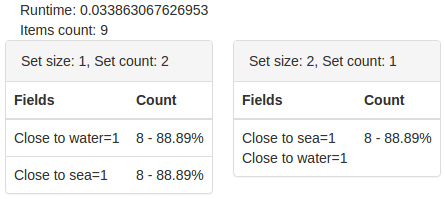
\includegraphics[width=0.5\textwidth]{images/tc1.png}
	\caption{TC1 - Ausgabe des Programmes}
	\label{fig:testingfazit:testing:testcases:1-1}
\end{figure}
\begin{table}[H] 
	\caption{TC2 Auswertung}
	\centering
	\label{fig:testingfazit:testing:testcases:2}
	\begin{tabular}{ | l | l | l | } 
		\hline 
		\rowcolor{tableheadcolor}
		\multicolumn{3}{|l|}{\bfseries ID: TC2} \\ \hline 
		Datebquelle & \multicolumn{2}{|l|}{\cref{app:testdatenquellen:2}} \\ \hline 
		Dateneinschränkung & \multicolumn{2}{|l|}{Keine} \\ \hline 
		
		\rowcolor{tableheadcolor}
		\multicolumn{3}{|l|}{\bfseries Erwartetes Resultat} \\ \hline 
		& Attributmenge & Anzahl \\ \hline 
		
		1er-Attributmenge & \tabitem Haustiere erlaubt & 8 \\ \cline{2-3} 
		& \tabitem Aircondition vorhanden & 8 \\ \hline 
		
		2er-Attributmenge & \tabitem Haustiere erlaubt & 8 \\
		& \tabitem Aircondition vorhanden & \\ \hline
		
		\rowcolor{tableheadcolor}
		\multicolumn{3}{|l|}{\bfseries Tatsächliches Resultat} \\ \hline 
		& Attributmenge & Anzahl \\ \hline 
		
		1er-Attributmenge & \tabitem Haustiere erlaubt & 8 \\ \cline{2-3} 
		& \tabitem Aircondition vorhanden & 8 \\ \hline 
		
		2er-Attributmenge & \tabitem Haustiere erlaubt & 8 \\
		& \tabitem Aircondition vorhanden & \\ \hline
		
		\rowcolor{tableheadcolor}
		\multicolumn{3}{|l|}{\bfseries Testergebnis} \\ \hline 
		\multicolumn{3}{|l|}{\cellcolor{green!25}} \\ \hline 
	\end{tabular}
\end{table}
\begin{figure}[H]
	\RawFloats
	\centering
	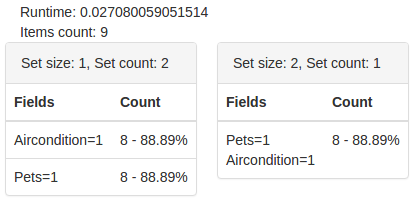
\includegraphics[width=0.5\textwidth]{images/tc2.png}
	\caption{TC2 - Ausgabe des Programmes}
	\label{fig:testingfazit:testing:testcases:2-1}
\end{figure}
\begin{table}[H] 
	\caption{TC3 Auswertung}
	\centering
	\label{fig:testingfazit:testing:testcases:3}
	\begin{tabular}{ | l | l | l | } 
		\hline 
		\rowcolor{tableheadcolor}
		\multicolumn{3}{|l|}{\bfseries ID: TC3} \\ \hline 
		Datebquelle & \multicolumn{2}{|l|}{\cref{app:testdatenquellen:3}} \\ \hline 
		Dateneinschränkung & \multicolumn{2}{|l|}{Keine} \\ \hline 
		
		\rowcolor{tableheadcolor}
		\multicolumn{3}{|l|}{\bfseries Erwartetes Resultat} \\ \hline 
		& Attributmenge & Anzahl \\ \hline 
		
		1er-Attributmenge & \tabitem Anzahl Zimmer=3 & 9 \\ \cline{2-3} 
		& \tabitem Anzahl Schlafzimmer=2 & 9 \\ \hline 
		
		2er-Attributmenge & \tabitem Anzahl Zimmer=3 & 9 \\
		& \tabitem Anzahl Schlafzimmer=2 & \\ \hline
		
		\rowcolor{tableheadcolor}
		\multicolumn{3}{|l|}{\bfseries Tatsächliches Resultat} \\ \hline 
		& Attributmenge & Anzahl \\ \hline 
		
		1er-Attributmenge & \tabitem Anzahl Zimmer=3 & 9 \\ \cline{2-3} 
		& \tabitem Anzahl Schlafzimmer=2 & 9 \\ \hline 
		
		2er-Attributmenge & \tabitem Anzahl Zimmer=3 & 9 \\
		& \tabitem Anzahl Schlafzimmer=2 & \\ \hline
		
		\rowcolor{tableheadcolor}
		\multicolumn{3}{|l|}{\bfseries Testergebnis} \\ \hline 
		\multicolumn{3}{|l|}{\cellcolor{green!25}} \\ \hline 
	\end{tabular}
\end{table}
\begin{figure}[H]
	\RawFloats
	\centering
	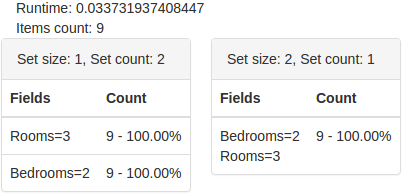
\includegraphics[width=0.5\textwidth]{images/tc3.png}
	\caption{TC3 - Ausgabe des Programmes}
	\label{fig:testingfazit:testing:testcases:3-1}
\end{figure}
\begin{table}[H] 
	\caption{TC4 Auswertung}
	\centering
	\label{fig:testingfazit:testing:testcases:4}
	\begin{tabular}{ | l | l | l | } 
		\hline 
		\rowcolor{tableheadcolor}
		\multicolumn{3}{|l|}{\bfseries ID: TC4} \\ \hline 
		Datebquelle & \multicolumn{2}{|l|}{\cref{app:testdatenquellen:4}} \\ \hline 
		Dateneinschränkung & \multicolumn{2}{|l|}{Keine} \\ \hline 
		
		\rowcolor{tableheadcolor}
		\multicolumn{3}{|l|}{\bfseries Erwartetes Resultat} \\ \hline 
		& Attributmenge & Anzahl \\ \hline 
		
		1er-Attributmenge & \tabitem Haustiere erlaubt & 8 \\ \cline{2-3} 
		& \tabitem Anzahl Schlafzimmer=3 & 9 \\ \hline 
		
		2er-Attributmenge & \tabitem Haustiere erlaubt & 8 \\
		& \tabitem Anzahl Schlafzimmer=3 & \\ \hline
		
		\rowcolor{tableheadcolor}
		\multicolumn{3}{|l|}{\bfseries Tatsächliches Resultat} \\ \hline 
		& Attributmenge & Anzahl \\ \hline 
		
		1er-Attributmenge & \tabitem Haustiere erlaubt & 8 \\ \cline{2-3} 
		& \tabitem Anzahl Schlafzimmer=3 & 9 \\ \hline 
		
		2er-Attributmenge & \tabitem Haustiere erlaubt & 8 \\
		& \tabitem Anzahl Schlafzimmer=3 & \\ \hline
		
		\rowcolor{tableheadcolor}
		\multicolumn{3}{|l|}{\bfseries Testergebnis} \\ \hline 
		\multicolumn{3}{|l|}{\cellcolor{green!25}} \\ \hline 
	\end{tabular}
\end{table}
\begin{figure}[H]
	\RawFloats
	\centering
	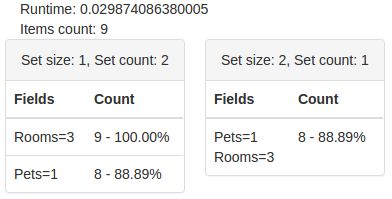
\includegraphics[width=0.5\textwidth]{images/tc4.png}
	\caption{TC4 - Ausgabe des Programmes}
	\label{fig:testingfazit:testing:testcases:4-1}
\end{figure}
\begin{table}[H] 
	\caption{TC5 Auswertung}
	\centering
	\label{fig:testingfazit:testing:testcases:5}
	\begin{tabular}{ | l | l | l | } 
		\hline 
		\rowcolor{tableheadcolor}
		\multicolumn{3}{|l|}{\bfseries ID: TC5} \\ \hline 
		Datebquelle & \multicolumn{2}{|l|}{\cref{app:testdatenquellen:5}} \\ \hline 
		Dateneinschränkung & \multicolumn{2}{|l|}{Haustiere erlaubt} \\ \hline 
		
		\rowcolor{tableheadcolor}
		\multicolumn{3}{|l|}{\bfseries Erwartetes Resultat} \\ \hline 
		& Attributmenge & Anzahl \\ \hline 
		
		1er-Attributmenge & \tabitem Nahe am Wasser & 4 \\ \cline{2-3} 
		& \tabitem Nahe am Meer & 5 \\ \hline 
		
		2er-Attributmenge & \tabitem Nahe am Wasser & 3 \\
		& \tabitem Nahe am Meer & \\ \hline
		
		\rowcolor{tableheadcolor}
		\multicolumn{3}{|l|}{\bfseries Tatsächliches Resultat} \\ \hline 
		& Attributmenge & Anzahl \\ \hline 
		
		1er-Attributmenge & \tabitem Nahe am Wasser & 4 \\ \cline{2-3} 
		& \tabitem Nahe am Meer & 5 \\ \hline 
		
		2er-Attributmenge & \tabitem Nahe am Wasser & 3 \\
		& \tabitem Nahe am Meer & \\ \hline
		
		\rowcolor{tableheadcolor}
		\multicolumn{3}{|l|}{\bfseries Testergebnis} \\ \hline 
		\multicolumn{3}{|l|}{\cellcolor{green!25}} \\ \hline 
	\end{tabular}
\end{table}
\begin{figure}[H]
	\RawFloats
	\centering
	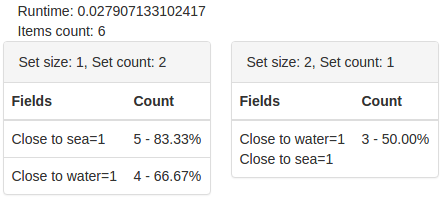
\includegraphics[width=0.5\textwidth]{images/tc5}
	\caption{TC5 - Ausgabe des Programmes}
	\label{fig:testingfazit:testing:testcases:5-1}
\end{figure}
\begin{table}[H] 
	\caption{TC6 Auswertung}
	\centering
	\label{fig:testingfazit:testing:testcases:6}
	\begin{tabular}{ | l | l | l | } 
		\hline 
		\rowcolor{tableheadcolor}
		\multicolumn{3}{|l|}{\bfseries ID: TC6} \\ \hline 
		Datebquelle & \multicolumn{2}{|l|}{\cref{app:testdatenquellen:6}} \\ \hline 
		Dateneinschränkung & \multicolumn{2}{|l|}{Nahe am ÖV (öffentlicher Verkehr)} \\ \hline 
		
		\rowcolor{tableheadcolor}
		\multicolumn{3}{|l|}{\bfseries Erwartetes Resultat} \\ \hline 
		& Attributmenge & Anzahl \\ \hline 
		
		1er-Attributmenge & \tabitem Nahe am Wasser & 3 \\ \cline{2-3} 
		& \tabitem Nahe am Meer & 4 \\ \hline 
		
		2er-Attributmenge & \tabitem Nahe am Wasser & 3 \\
		& \tabitem Nahe am Meer & \\ \hline
		
		\rowcolor{tableheadcolor}
		\multicolumn{3}{|l|}{\bfseries Tatsächliches Resultat} \\ \hline 
		& Attributmenge & Anzahl \\ \hline 
		
		1er-Attributmenge & \tabitem Nahe am Wasser & 3 \\ \cline{2-3} 
		& \tabitem Nahe am Meer & 4 \\ \hline 
		
		2er-Attributmenge & \tabitem Nahe am Wasser & 3 \\
		& \tabitem Nahe am Meer & \\ \hline
		
		\rowcolor{tableheadcolor}
		\multicolumn{3}{|l|}{\bfseries Testergebnis} \\ \hline 
		\multicolumn{3}{|l|}{\cellcolor{green!25}} \\ \hline 
	\end{tabular}
\end{table}
\begin{figure}[H]
	\RawFloats
	\centering
	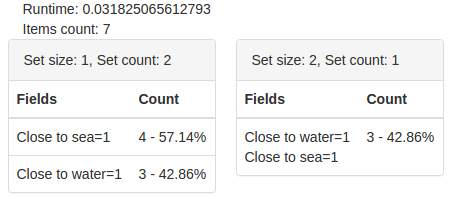
\includegraphics[width=0.5\textwidth]{images/tc6.png}
	\caption{TC6 - Ausgabe des Programmes}
	\label{fig:testingfazit:testing:testcases:6-1}
\end{figure}
\begin{table}[H] 
	\caption{TC7 Auswertung}
	\centering
	\label{fig:testingfazit:testing:testcases:7}
	\begin{tabular}{ | l | l | l | } 
		\hline 
		\rowcolor{tableheadcolor}
		\multicolumn{3}{|l|}{\bfseries ID: TC7} \\ \hline 
		Datebquelle & \multicolumn{2}{|l|}{\cref{app:testdatenquellen:7}} \\ \hline 
		Dateneinschränkung & \multicolumn{2}{|l|}{Anzahl Zimmer=3} \\ \hline 
		
		\rowcolor{tableheadcolor}
		\multicolumn{3}{|l|}{\bfseries Erwartetes Resultat} \\ \hline 
		& Attributmenge & Anzahl \\ \hline 
		
		1er-Attributmenge & \tabitem Nahe am Wasser & 6 \\ \cline{2-3} 
		& \tabitem Nahe am Meer & 4 \\ \hline 
		
		2er-Attributmenge & \tabitem Nahe am Wasser & 4 \\
		& \tabitem Nahe am Meer & \\ \hline
		
		\rowcolor{tableheadcolor}
		\multicolumn{3}{|l|}{\bfseries Tatsächliches Resultat} \\ \hline 
		& Attributmenge & Anzahl \\ \hline 
		
		1er-Attributmenge & \tabitem Nahe am Wasser & 6 \\ \cline{2-3} 
		& \tabitem Nahe am Meer & 4 \\ \hline 
		
		2er-Attributmenge & \tabitem Nahe am Wasser & 4 \\
		& \tabitem Nahe am Meer & \\ \hline
		
		\rowcolor{tableheadcolor}
		\multicolumn{3}{|l|}{\bfseries Testergebnis} \\ \hline 
		\multicolumn{3}{|l|}{\cellcolor{green!25}} \\ \hline 
	\end{tabular}
\end{table}
\begin{figure}[H]
	\RawFloats
	\centering
	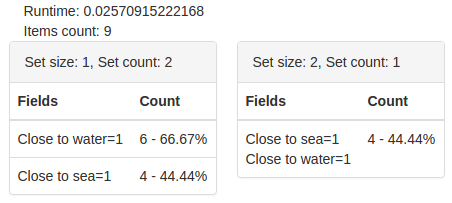
\includegraphics[width=0.5\textwidth]{images/tc7.png}
	\caption{TC7 - Ausgabe des Programmes}
	\label{fig:testingfazit:testing:testcases:7-1}
\end{figure}
\begin{table}[H] 
	\caption{TC8 Auswertung}
	\centering
	\label{fig:testingfazit:testing:testcases:8}
	\begin{tabular}{ | l | l | l | } 
		\hline 
		\rowcolor{tableheadcolor}
		\multicolumn{3}{|l|}{\bfseries ID: TC8} \\ \hline 
		Datebquelle & \multicolumn{2}{|l|}{\cref{app:testdatenquellen:8}} \\ \hline 
		Dateneinschränkung & \multicolumn{2}{|l|}{Keine} \\ \hline 
		
		\rowcolor{tableheadcolor}
		\multicolumn{3}{|l|}{\bfseries Erwartetes Resultat} \\ \hline 
		& Attributmenge & Anzahl \\ \hline 
		
		1er-Attributmenge & \tabitem Nahe am Wasser & 14 \\ \cline{2-3} 
		& \tabitem Nahe am Meer & 13 \\ \cline{2-3} 
		& \tabitem Haustiere erlaubt & 12 \\ \hline 
		
		2er-Attributmenge & \tabitem Nahe am Wasser & 11 \\
		& \tabitem Nahe am Meer & \\ \cline{2-3} 
		& \tabitem Nahe am Wasser & 10 \\
		& \tabitem Haustiere erlaubt & \\ \cline{2-3} 
		& \tabitem Nahe am Meer & 9 \\
		& \tabitem Haustiere erlaubt & \\ \hline
		
		3er-Attributmenge & \tabitem Nahe am Wasser & 8 \\
		& \tabitem Nahe am Meer & \\ 
		& \tabitem Haustiere erlaubt & \\ \hline
		
		\rowcolor{tableheadcolor}
		\multicolumn{3}{|l|}{\bfseries Tatsächliches Resultat} \\ \hline 
		& Attributmenge & Anzahl \\ \hline 
		
		1er-Attributmenge & \tabitem Nahe am Wasser & 14 \\ \cline{2-3} 
		& \tabitem Nahe am Meer & 13 \\ \cline{2-3} 
		& \tabitem Haustiere erlaubt & 12 \\ \hline 
		
		2er-Attributmenge & \tabitem Nahe am Wasser & 11 \\
		& \tabitem Nahe am Meer & \\ \cline{2-3} 
		& \tabitem Nahe am Wasser & 10 \\
		& \tabitem Haustiere erlaubt & \\ \cline{2-3} 
		& \tabitem Nahe am Meer & 9 \\
		& \tabitem Haustiere erlaubt & \\ \hline
		
		3er-Attributmenge & \tabitem Nahe am Wasser & 8 \\
		& \tabitem Nahe am Meer & \\ 
		& \tabitem Haustiere erlaubt & \\ \hline
		
		\rowcolor{tableheadcolor}
		\multicolumn{3}{|l|}{\bfseries Testergebnis} \\ \hline 
		\multicolumn{3}{|l|}{\cellcolor{green!25}} \\ \hline 
	\end{tabular}
\end{table}
\begin{figure}[H]
	\RawFloats
	\centering
	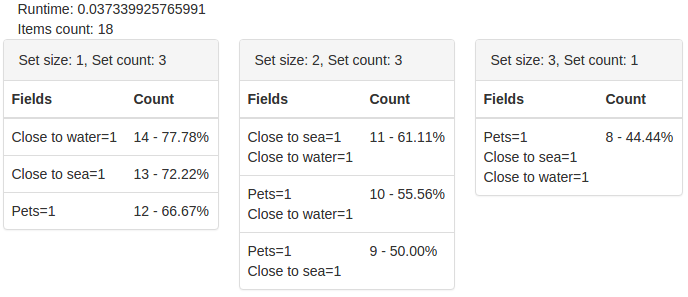
\includegraphics[width=1\textwidth]{images/tc8.png}
	\caption{TC8 - Ausgabe des Programmes}
	\label{fig:testingfazit:testing:testcases:8-1}
\end{figure}
\begin{table}[H] 
	\caption{TC9 Auswertung}
	\centering
	\label{fig:testingfazit:testing:testcases:9}
	\begin{tabular}{ | l | l | l | } 
		\hline 
		\rowcolor{tableheadcolor}
		\multicolumn{3}{|l|}{\bfseries ID: TC9} \\ \hline 
		Datebquelle & \multicolumn{2}{|l|}{\cref{app:testdatenquellen:9}} \\ \hline 
		Dateneinschränkung & \multicolumn{2}{|l|}{Keine} \\ \hline 
		
		\rowcolor{tableheadcolor}
		\multicolumn{3}{|l|}{\bfseries Erwartetes Resultat} \\ \hline 
		& Attributmenge & Anzahl \\ \hline 
		
		1er-Attributmenge & \tabitem Nahe am Wasser & 8 \\ \cline{2-3} 
		& \tabitem Nahe am Meer & 8 \\ \cline{2-3} 
		& \tabitem Haustiere erlaubt & 9 \\ \cline{2-3} 
		& \tabitem Anzahl Zimmer=3 & 11 \\ \hline
		
		2er-Attributmenge & \tabitem Nahe am Wasser & 8 \\
		& \tabitem Nahe am Meer & \\ \cline{2-3} 
		& \tabitem Haustiere erlaubt & 9 \\
		& \tabitem Anzahl Zimmer=3 & \\ \hline
		
		\rowcolor{tableheadcolor}
		\multicolumn{3}{|l|}{\bfseries Tatsächliches Resultat} \\ \hline 
		& Attributmenge & Anzahl \\ \hline 
		
		1er-Attributmenge & \tabitem Nahe am Wasser & 8 \\ \cline{2-3} 
		& \tabitem Nahe am Meer & 8 \\ \cline{2-3} 
		& \tabitem Haustiere erlaubt & 9 \\ \cline{2-3} 
		& \tabitem Anzahl Zimmer=3 & 11 \\ \hline
		
		2er-Attributmenge & \tabitem Nahe am Wasser & 8 \\
		& \tabitem Nahe am Meer & \\ \cline{2-3} 
		& \tabitem Haustiere erlaubt & 9 \\
		& \tabitem Anzahl Zimmer=3 & \\ \hline
		
		\rowcolor{tableheadcolor}
		\multicolumn{3}{|l|}{\bfseries Testergebnis} \\ \hline 
		\multicolumn{3}{|l|}{\cellcolor{green!25}} \\ \hline 
	\end{tabular}
\end{table}
\begin{figure}[H]
	\RawFloats
	\centering
	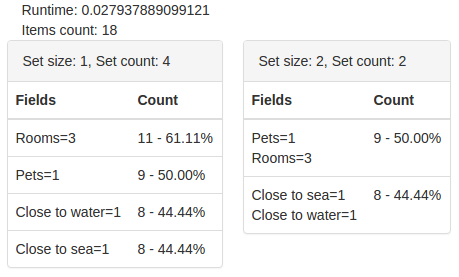
\includegraphics[width=0.5\textwidth]{images/tc9.png}
	\caption{TC9 - Ausgabe des Programmes}
	\label{fig:testingfazit:testing:testcases:9-1}
\end{figure}
\begin{longtable}{ | l | l | l | l |} 	
	\hline 
	\rowcolor{tableheadcolor}
	\multicolumn{4}{|l|}{\bfseries ID: TC10} \\ \hline 
	Datebquelle & \multicolumn{3}{|l|}{\cref{app:testdatenquellen:10}} \\ \hline 
	Dateneinschränkung & \multicolumn{3}{|l|}{Keine} \\ \hline 
	
	\rowcolor{tableheadcolor}
	\multicolumn{4}{|l|}{\bfseries Erwartetes Resultat} \\ \hline 
	Noise Punkte & \multicolumn{3}{|l|}{0} \\ \hline 
	
	% ----------------------------------------------		
	\multicolumn{4}{|l|}{\textbf{Cluster 1}} \\ \cline{2-4} 
	& Fehler & \multicolumn{2}{|l|}{0} \\ \cline{2-4} 
	& Grösse & \multicolumn{2}{|l|}{5} \\ \cline{2-4} 
	&& Attributmenge & Anzahl \\ \cline{2-4} 
	
	& 1er-Attributmenge & \tabitem Nahe am Wasser & 5 \\ \cline{3-4} 
	& & \tabitem Nahe am Meer & 5 \\ \cline{3-4} 
	& & \tabitem Anzahl Zimmer=3 & 5 \\ \cline{3-4} 
	& & \tabitem Anzahl Schlafzimmer=2 & 5 \\ \cline{2-4} 
	
	& 2er-Attributmenge & \tabitem Nahe am Wasser & 5 \\
	& & \tabitem Nahe am Meer & \\ \cline{3-4} 
	& & \tabitem Nahe am Wasser & 5 \\
	& & \tabitem Anzahl Zimmer=3 & \\ \cline{3-4} 
	& & \tabitem Nahe am Wasser & 5 \\
	& & \tabitem Anzahl Schlafzimmer=2 & \\ \cline{3-4} 
	
	& & \tabitem Nahe am Meer & 5 \\
	& & \tabitem Anzahl Zimmer=3 & \\ \cline{3-4} 
	& & \tabitem Nahe am Meer & 5 \\
	& & \tabitem Anzahl Schlafzimmer=2 & \\ \cline{3-4} 
	
	& & \tabitem Anzahl Zimmer=3 & 5 \\
	& & \tabitem Anzahl Schlafzimmer=2 & \\ \cline{2-4} 
	
	& 3er-Attributmenge & \tabitem Nahe am Wasser & 5 \\
	& & \tabitem Nahe am Meer & \\ 
	& & \tabitem Anzahl Zimmer=3 & \\ \cline{3-4} 
	& & \tabitem Nahe am Wasser & 5 \\
	& & \tabitem Nahe am Meer & \\ 
	& & \tabitem Anzahl Schlafzimmer=2 & \\ \cline{3-4}
	& & \tabitem Nahe am Meer & 5 \\
	& & \tabitem Anzahl Zimmer=3 & \\ 
	& & \tabitem Anzahl Schlafzimmer=2 & \\ \cline{3-4}
	& & \tabitem Nahe am Wasser & 5 \\
	& & \tabitem Anzahl Zimmer=3 & \\ 
	& & \tabitem Anzahl Schlafzimmer=2 & \\ \cline{2-4}
	
	& 4er-Attributmenge & \tabitem Nahe am Wasser & 5 \\
	& & \tabitem Nahe am Meer & \\ 
	& & \tabitem Anzahl Zimmer=3 & \\ 
	& & \tabitem Anzahl Schlafzimmer=2 & \\ \hline
	
	% ----------------------------------------------
	\multicolumn{4}{|l|}{\textbf{Cluster 2}} \\ \cline{2-4} 
	& Fehler & \multicolumn{2}{|l|}{0} \\ \cline{2-4} 
	& Grösse & \multicolumn{2}{|l|}{4} \\ \cline{2-4} 
	& & Attributmenge & Anzahl \\ \cline{2-4} 
	
	& 1er-Attributmenge & \tabitem Wochenpreis=günstig & 4 \\ \cline{3-4}
	& & \tabitem Anzahl Zimmer=9 & 4 \\ \cline{3-4}
	& & \tabitem Anzahl Schlafzimmer=9 & 4 \\ \cline{2-4} 
	
	& 2er-Attributmenge & \tabitem Wochenpreis=günstig & 4 \\
	& & \tabitem Anzahl Zimmer=9 & \\ \cline{3-4}
	& & \tabitem Wochenpreis=günstig & 4 \\
	& & \tabitem Anzahl Schlafzimmer=9 & \\ \cline{3-4} 
	& & \tabitem Anzahl Zimmer=9 & 4 \\
	& & \tabitem Anzahl Schlafzimmer=9 & \\ \cline{2-4}
	
	& 3er-Attributmenge & \tabitem Wochenpreis=günstig & 4 \\
	& & \tabitem Anzahl Zimmer=9 & \\ 
	& & \tabitem Anzahl Schlafzimmer=9 & \\ \hline
	
	\rowcolor{tableheadcolor}
	\multicolumn{4}{|l|}{\bfseries Tatsächliches Resultat} \\ \hline 
	Noise Punkte & \multicolumn{3}{|l|}{0} \\ \hline 
	
	% ----------------------------------------------		
	\multicolumn{4}{|l|}{\textbf{Cluster 1}} \\ \cline{2-4} 
	& Fehler & \multicolumn{2}{|l|}{0} \\ \cline{2-4} 
	& Grösse & \multicolumn{2}{|l|}{5} \\ \cline{2-4} 
	&& Attributmenge & Anzahl \\ \cline{2-4} 
	
	& 1er-Attributmenge & \tabitem Nahe am Wasser & 5 \\ \cline{3-4} 
	& & \tabitem Nahe am Meer & 5 \\ \cline{3-4} 
	& & \tabitem Anzahl Zimmer=3 & 5 \\ \cline{3-4} 
	& & \tabitem Anzahl Schlafzimmer=2 & 5 \\ \cline{2-4} 
	
	& 2er-Attributmenge & \tabitem Nahe am Wasser & 5 \\
	& & \tabitem Nahe am Meer & \\ \cline{3-4} 
	& & \tabitem Nahe am Wasser & 5 \\
	& & \tabitem Anzahl Zimmer=3 & \\ \cline{3-4} 
	& & \tabitem Nahe am Wasser & 5 \\
	& & \tabitem Anzahl Schlafzimmer=2 & \\ \cline{3-4} 
	
	& & \tabitem Nahe am Meer & 5 \\
	& & \tabitem Anzahl Zimmer=3 & \\ \cline{3-4} 
	& & \tabitem Nahe am Meer & 5 \\
	& & \tabitem Anzahl Schlafzimmer=2 & \\ \cline{3-4} 
	
	& & \tabitem Anzahl Zimmer=3 & 5 \\
	& & \tabitem Anzahl Schlafzimmer=2 & \\ \cline{2-4} 
	
	& 3er-Attributmenge & \tabitem Nahe am Wasser & 5 \\
	& & \tabitem Nahe am Meer & \\ 
	& & \tabitem Anzahl Zimmer=3 & \\ \cline{3-4} 
	& & \tabitem Nahe am Wasser & 5 \\
	& & \tabitem Nahe am Meer & \\ 
	& & \tabitem Anzahl Schlafzimmer=2 & \\ \cline{3-4}
	& & \tabitem Nahe am Meer & 5 \\
	& & \tabitem Anzahl Zimmer=3 & \\ 
	& & \tabitem Anzahl Schlafzimmer=2 & \\ \cline{3-4}
	& & \tabitem Nahe am Wasser & 5 \\
	& & \tabitem Anzahl Zimmer=3 & \\ 
	& & \tabitem Anzahl Schlafzimmer=2 & \\ \cline{2-4}
	
	& 4er-Attributmenge & \tabitem Nahe am Wasser & 5 \\
	& & \tabitem Nahe am Meer & \\ 
	& & \tabitem Anzahl Zimmer=3 & \\ 
	& & \tabitem Anzahl Schlafzimmer=2 & \\ \hline
	
	% ----------------------------------------------
	\multicolumn{4}{|l|}{\textbf{Cluster 2}} \\ \cline{2-4} 
	& Fehler & \multicolumn{2}{|l|}{0} \\ \cline{2-4} 
	& Grösse & \multicolumn{2}{|l|}{4} \\ \cline{2-4} 
	& & Attributmenge & Anzahl \\ \cline{2-4} 
	
	& 1er-Attributmenge & \tabitem Wochenpreis=günstig & 4 \\ \cline{3-4}
	& & \tabitem Anzahl Zimmer=9 & 4 \\ \cline{3-4}
	& & \tabitem Anzahl Schlafzimmer=9 & 4 \\ \cline{2-4} 
	
	& 2er-Attributmenge & \tabitem Wochenpreis=günstig & 4 \\
	& & \tabitem Anzahl Zimmer=9 & \\ \cline{3-4}
	& & \tabitem Wochenpreis=günstig & 4 \\
	& & \tabitem Anzahl Schlafzimmer=9 & \\ \cline{3-4} 
	& & \tabitem Anzahl Zimmer=9 & 4 \\
	& & \tabitem Anzahl Schlafzimmer=9 & \\ \cline{2-4}
	
	& 3er-Attributmenge & \tabitem Wochenpreis=günstig & 4 \\
	& & \tabitem Anzahl Zimmer=9 & \\ 
	& & \tabitem Anzahl Schlafzimmer=9 & \\ \hline
	
	\rowcolor{tableheadcolor}
	\multicolumn{4}{|l|}{\bfseries Testergebnis} \\ \hline 
	\multicolumn{4}{|l|}{\cellcolor{green!25}} \\ \hline 
	
	\caption{TC10 Auswertung}
	\centering
	\label{fig:testingfazit:testing:testcases:10}
\end{longtable}
\begin{figure}[H]
	\begin{subfigure}[t]{1\textwidth}
		\centering
		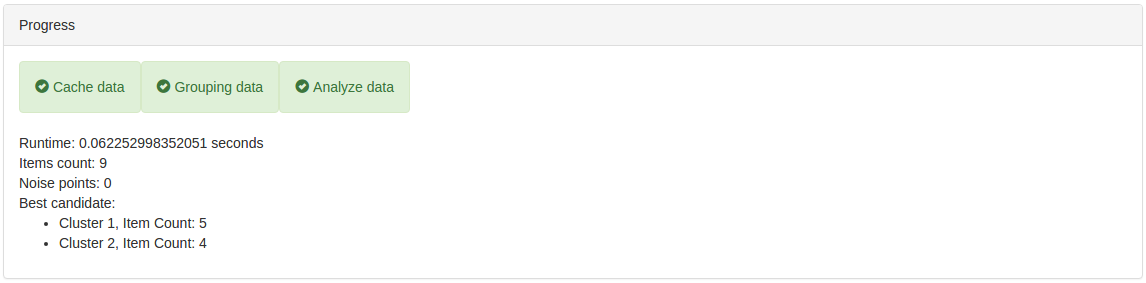
\includegraphics[width=1\textwidth]{images/tc10-dbscan-1}
		\caption{Generelle Informationen}
		\label{fig:testingfazit:testing:testcases:10-1-1}
	\end{subfigure} \\
	\begin{subfigure}[t]{1\textwidth}
		\centering
		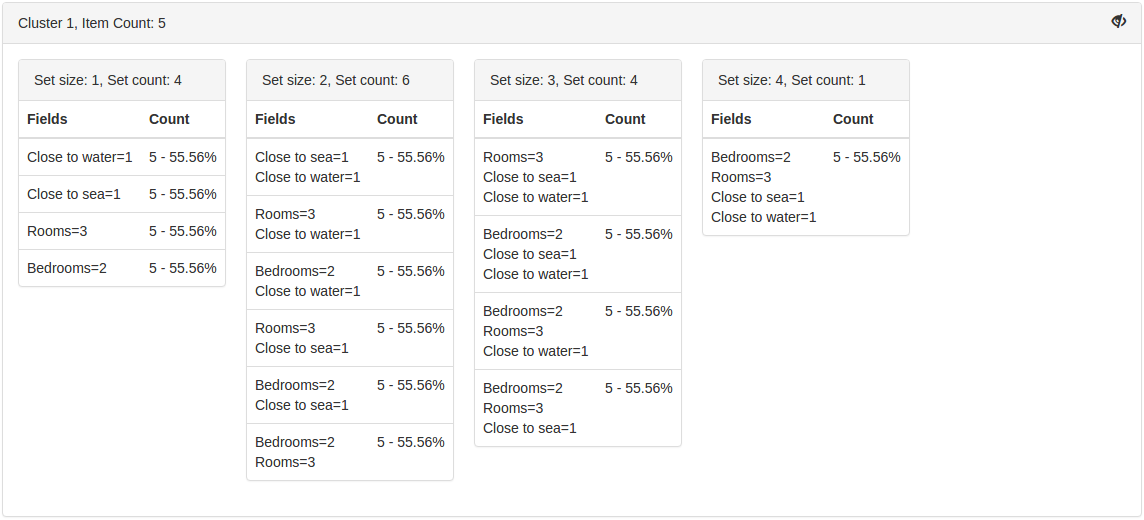
\includegraphics[width=1\textwidth]{images/tc10-dbscan-2}
		\caption{Cluster 1}
		\label{fig:testingfazit:testing:testcases:10-1-2}
	\end{subfigure}
	\begin{subfigure}[t]{1\textwidth}
		\centering
		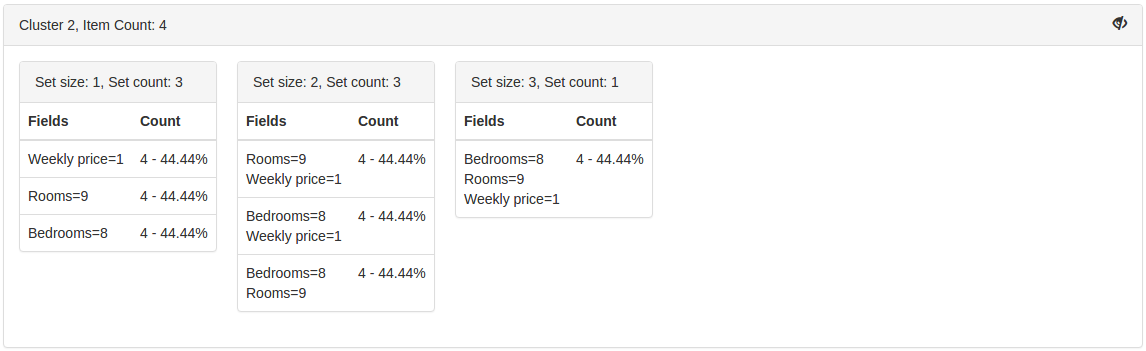
\includegraphics[width=1\textwidth]{images/tc10-dbscan-3}
		\caption{Cluster 2}
		\label{fig:testingfazit:testing:testcases:10-1-3}
	\end{subfigure}
	\caption{TC10 - Ausgabe des Programmes - Resultat des DBSCAN Algorithmus}
	\label{fig:testingfazit:testing:testcases:10-1}
\end{figure}
\begin{figure}[H]
	\begin{subfigure}[t]{1\textwidth}
		\centering
		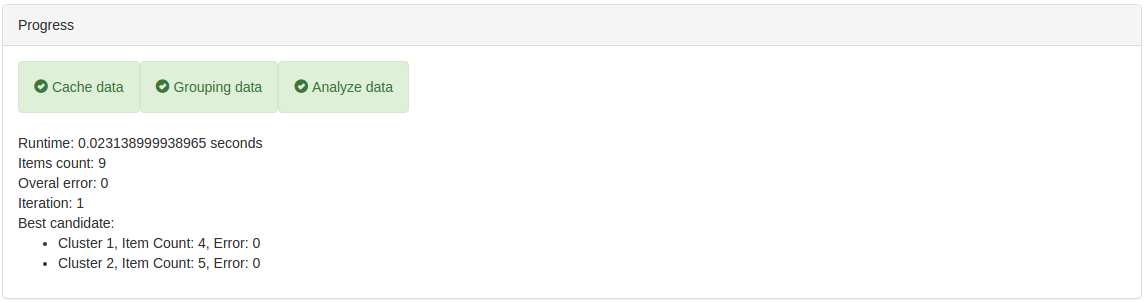
\includegraphics[width=1\textwidth]{images/tc10-kprototype-1}
		\caption{Generelle Informationen}
		\label{fig:testingfazit:testing:testcases:10-2-1}
	\end{subfigure} \\
	\begin{subfigure}[t]{1\textwidth}
		\centering
		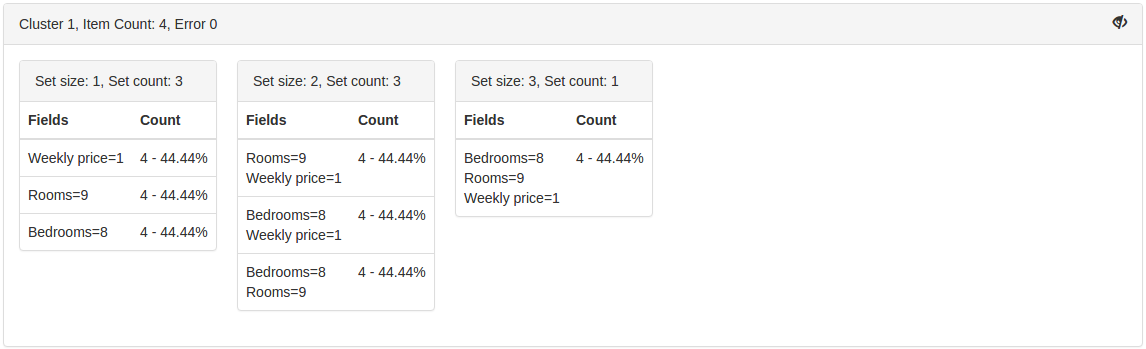
\includegraphics[width=1\textwidth]{images/tc10-kprototype-2}
		\caption{Cluster 1}
		\label{fig:testingfazit:testing:testcases:10-2-2}
	\end{subfigure}
	\begin{subfigure}[t]{1\textwidth}
		\centering
		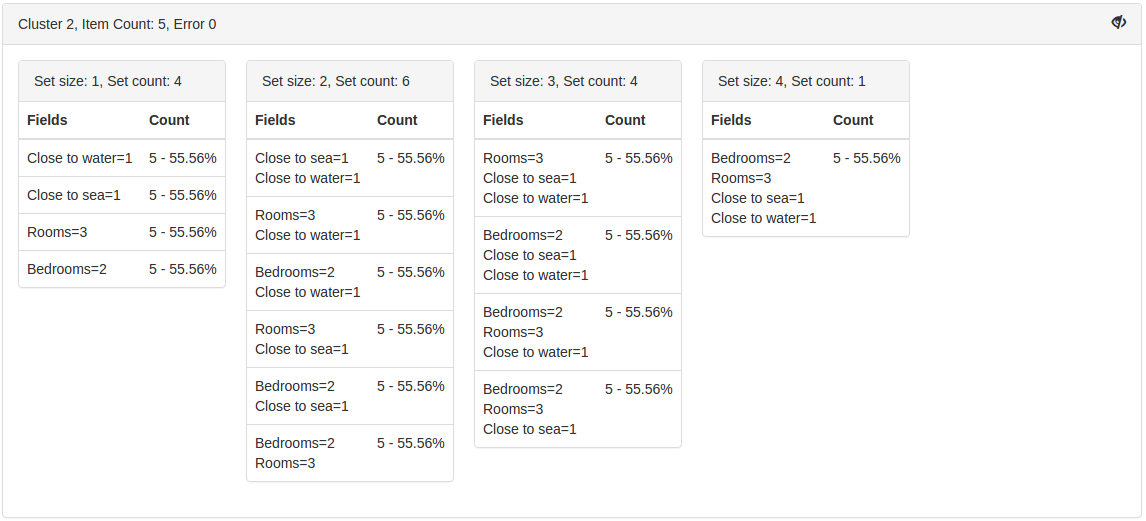
\includegraphics[width=1\textwidth]{images/tc10-kprototype-3}
		\caption{Cluster 2}
		\label{fig:testingfazit:testing:testcases:10-2-3}
	\end{subfigure}
	\caption{TC10 - Ausgabe des Programmes - Resultat des k-prototype Algorithmus}
	\label{fig:testingfazit:testing:testcases:10-2}
\end{figure}
\begin{longtable}{ | l | l | l | l |} 	
	\hline 
	\rowcolor{tableheadcolor}
	\multicolumn{4}{|l|}{\bfseries ID: TC11-1 DBSCAN} \\ \hline 
	Datebquelle & \multicolumn{3}{|l|}{\cref{app:testdatenquellen:11}} \\ \hline 
	Dateneinschränkung & \multicolumn{3}{|l|}{Keine} \\ \hline 
	
	\rowcolor{tableheadcolor}
	\multicolumn{4}{|l|}{\bfseries Erwartetes Resultat} \\ \hline 
	Noise Punkte & \multicolumn{3}{|l|}{1} \\ \hline 
	
	% ----------------------------------------------		
	\multicolumn{4}{|l|}{\textbf{Cluster 1}} \\ \cline{2-4} 
	& Grösse & \multicolumn{2}{|l|}{9} \\ \cline{2-4} 
	&& Attributmenge & Anzahl \\ \cline{2-4} 
	
	& 1er-Attributmenge & \tabitem Nahe am Wasser & 9 \\ \cline{3-4} 
	& & \tabitem Nahe am Meer & 9 \\ \cline{3-4} 
	& & \tabitem Anzahl Zimmer=3 & 9 \\ \cline{3-4} 
	& & \tabitem Anzahl Schlafzimmer=2 & 9 \\ \cline{2-4} 
	
	& 2er-Attributmenge & \tabitem Nahe am Wasser & 9 \\
	& & \tabitem Nahe am Meer & \\ \cline{3-4} 
	& & \tabitem Nahe am Wasser & 9 \\
	& & \tabitem Anzahl Zimmer=3 & \\ \cline{3-4} 
	& & \tabitem Nahe am Wasser & 9 \\
	& & \tabitem Anzahl Schlafzimmer=2 & \\ \cline{3-4} 
	
	& & \tabitem Nahe am Meer & 9 \\
	& & \tabitem Anzahl Zimmer=3 & \\ \cline{3-4} 
	& & \tabitem Nahe am Meer & 9 \\
	& & \tabitem Anzahl Schlafzimmer=2 & \\ \cline{3-4} 
	
	& & \tabitem Anzahl Zimmer=3 & 9 \\
	& & \tabitem Anzahl Schlafzimmer=2 & \\ \cline{2-4} 
	
	& 3er-Attributmenge & \tabitem Nahe am Wasser & 9 \\
	& & \tabitem Nahe am Meer & \\ 
	& & \tabitem Anzahl Zimmer=3 & \\ \cline{3-4} 
	& & \tabitem Nahe am Wasser & 9 \\
	& & \tabitem Nahe am Meer & \\ 
	& & \tabitem Anzahl Schlafzimmer=2 & \\ \cline{3-4}
	& & \tabitem Nahe am Meer & 9 \\
	& & \tabitem Anzahl Zimmer=3 & \\ 
	& & \tabitem Anzahl Schlafzimmer=2 & \\ \cline{3-4}
	& & \tabitem Nahe am Wasser & 9 \\
	& & \tabitem Anzahl Zimmer=3 & \\ 
	& & \tabitem Anzahl Schlafzimmer=2 & \\ \cline{2-4}
	
	& 4er-Attributmenge & \tabitem Nahe am Wasser & 9 \\
	& & \tabitem Nahe am Meer & \\ 
	& & \tabitem Anzahl Zimmer=3 & \\ 
	& & \tabitem Anzahl Schlafzimmer=2 & \\ \hline
	
	\rowcolor{tableheadcolor}
	\multicolumn{4}{|l|}{\bfseries Tatsächliches Resultat} \\ \hline 
	Noise Punkte & \multicolumn{3}{|l|}{1} \\ \hline 
	
	% ----------------------------------------------		
	\multicolumn{4}{|l|}{\textbf{Cluster 1}} \\ \cline{2-4} 
	& Grösse & \multicolumn{2}{|l|}{9} \\ \cline{2-4} 
	&& Attributmenge & Anzahl \\ \cline{2-4} 
	
	& 1er-Attributmenge & \tabitem Nahe am Wasser & 9 \\ \cline{3-4} 
	& & \tabitem Nahe am Meer & 9 \\ \cline{3-4} 
	& & \tabitem Anzahl Zimmer=3 & 9 \\ \cline{3-4} 
	& & \tabitem Anzahl Schlafzimmer=2 & 9 \\ \cline{2-4} 
	
	& 2er-Attributmenge & \tabitem Nahe am Wasser & 9 \\
	& & \tabitem Nahe am Meer & \\ \cline{3-4} 
	& & \tabitem Nahe am Wasser & 9 \\
	& & \tabitem Anzahl Zimmer=3 & \\ \cline{3-4} 
	& & \tabitem Nahe am Wasser & 9 \\
	& & \tabitem Anzahl Schlafzimmer=2 & \\ \cline{3-4} 
	
	& & \tabitem Nahe am Meer & 9 \\
	& & \tabitem Anzahl Zimmer=3 & \\ \cline{3-4} 
	& & \tabitem Nahe am Meer & 9 \\
	& & \tabitem Anzahl Schlafzimmer=2 & \\ \cline{3-4} 
	
	& & \tabitem Anzahl Zimmer=3 & 9 \\
	& & \tabitem Anzahl Schlafzimmer=2 & \\ \cline{2-4} 
	
	& 3er-Attributmenge & \tabitem Nahe am Wasser & 9 \\
	& & \tabitem Nahe am Meer & \\ 
	& & \tabitem Anzahl Zimmer=3 & \\ \cline{3-4} 
	& & \tabitem Nahe am Wasser & 9 \\
	& & \tabitem Nahe am Meer & \\ 
	& & \tabitem Anzahl Schlafzimmer=2 & \\ \cline{3-4}
	& & \tabitem Nahe am Meer & 9 \\
	& & \tabitem Anzahl Zimmer=3 & \\ 
	& & \tabitem Anzahl Schlafzimmer=2 & \\ \cline{3-4}
	& & \tabitem Nahe am Wasser & 9 \\
	& & \tabitem Anzahl Zimmer=3 & \\ 
	& & \tabitem Anzahl Schlafzimmer=2 & \\ \cline{2-4}
	
	& 4er-Attributmenge & \tabitem Nahe am Wasser & 9 \\
	& & \tabitem Nahe am Meer & \\ 
	& & \tabitem Anzahl Zimmer=3 & \\ 
	& & \tabitem Anzahl Schlafzimmer=2 & \\ \hline
	
	\rowcolor{tableheadcolor}
	\multicolumn{4}{|l|}{\bfseries Testergebnis} \\ \hline 
	\multicolumn{4}{|l|}{\cellcolor{green!25}} \\ \hline 
	
	\caption{TC11-1 Auswertung vom DBSCAN Algorithmus}
	\centering
	\label{fig:testingfazit:testing:testcases:11:1}
\end{longtable}
\begin{figure}[H]
	\begin{subfigure}[t]{1\textwidth}
		\centering
		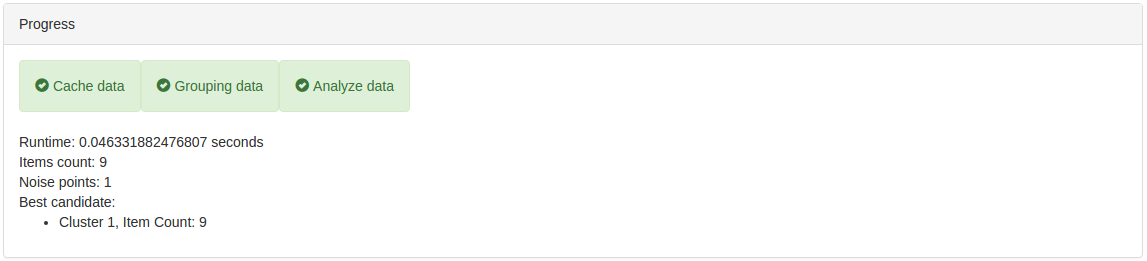
\includegraphics[width=1\textwidth]{images/tc11-dbscan-1}
		\caption{Generelle Informationen}
		\label{fig:testingfazit:testing:testcases:11-1-1}
	\end{subfigure} \\
	\begin{subfigure}[t]{1\textwidth}
		\centering
		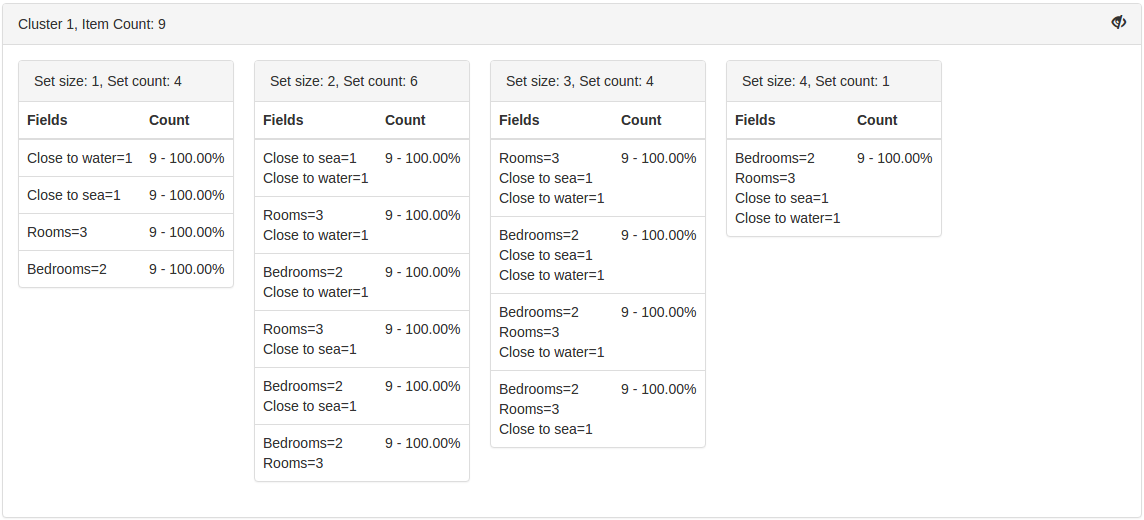
\includegraphics[width=1\textwidth]{images/tc11-dbscan-2}
		\caption{Cluster 1}
		\label{fig:testingfazit:testing:testcases:11-1-2}
	\end{subfigure}
	\caption{TC11 - Ausgabe des Programmes - Resultat des DBSCAN Algorithmus}
	\label{fig:testingfazit:testing:testcases:11-1}
\end{figure}

\begin{longtable}{ | l | l | l | l |} 	
	\hline 
	\rowcolor{tableheadcolor}
	\multicolumn{4}{|l|}{\bfseries ID: TC11-2 k-prototype} \\ \hline 
	Datebquelle & \multicolumn{3}{|l|}{\cref{app:testdatenquellen:11}} \\ \hline 
	Dateneinschränkung & \multicolumn{3}{|l|}{Keine} \\ \hline 
	
	\rowcolor{tableheadcolor}
	\multicolumn{4}{|l|}{\bfseries Erwartetes Resultat} \\ \hline 
	
	\multicolumn{4}{|l|}{\textbf{Cluster 1}} \\ \cline{2-4} 
	& Fehler & \multicolumn{2}{|l|}{0} \\ \cline{2-4} 
	& Grösse & \multicolumn{2}{|l|}{9} \\ \cline{2-4} 
	& \multicolumn{3}{|L{7.5cm}|}{Das Resultat der Analyse dieses Clusters vom Apriori Algorithmus ist dasselbe wie jenes vom DBSCAN welches oben aufgeführt wurde. Zur Verbesserung der Übersicht wird das Resultat hier nicht noch einmal aufgeführt.} \\ \hline
	
	\multicolumn{4}{|l|}{\textbf{Cluster 2}} \\ \cline{2-4} 
	& Fehler & \multicolumn{2}{|l|}{0} \\ \cline{2-4} 
	& Grösse & \multicolumn{2}{|l|}{1} \\ \cline{2-4} 
	& \multicolumn{3}{|L{7.5cm}|}{Der Apriori Algorithmus findet keine häufigen Attribute, da $minsup$ auf 0.2 (oder 20\%) gesetzt ist und nur 1 Element in diesem Cluster vorhanden ist.} \\ \hline
	
	
	\rowcolor{tableheadcolor}
	\multicolumn{4}{|l|}{\bfseries Tatsächliches Resultat} \\ \hline 
	
	\multicolumn{4}{|l|}{\textbf{Cluster 1}} \\ \cline{2-4} 
	& Fehler & \multicolumn{2}{|l|}{0} \\ \cline{2-4} 
	& Grösse & \multicolumn{2}{|l|}{9} \\ \cline{2-4} 
	& \multicolumn{3}{|L{7.5cm}|}{Das Resultat der Analyse dieses Clusters vom Apriori Algorithmus ist dasselbe wie jenes vom DBSCAN welches oben aufgeführt wurde. Zur Verbesserung der Übersicht wird das Resultat hier nicht noch einmal aufgeführt.} \\ \hline
	
	\multicolumn{4}{|l|}{\textbf{Cluster 2}} \\ \cline{2-4} 
	& Fehler & \multicolumn{2}{|l|}{0} \\ \cline{2-4} 
	& Grösse & \multicolumn{2}{|l|}{1} \\ \cline{2-4} 
	& \multicolumn{3}{|L{7.5cm}|}{Der Apriori Algorithmus findet keine häufigen Attribute, da $minsup$ auf 0.2 (oder 20\%) gesetzt ist und nur 1 Element in diesem Cluster vorhanden ist.} \\ \hline
	
	\rowcolor{tableheadcolor}
	\multicolumn{4}{|l|}{\bfseries Testergebnis} \\ \hline 
	\multicolumn{4}{|l|}{\cellcolor{green!25}} \\ \hline 
	
	\caption{TC11-2 Auswertung vom k-prototype Algorithmus}
	\centering
	\label{fig:testingfazit:testing:testcases:11:2}
\end{longtable}
\begin{figure}[H]
	\begin{subfigure}[t]{1\textwidth}
		\centering
		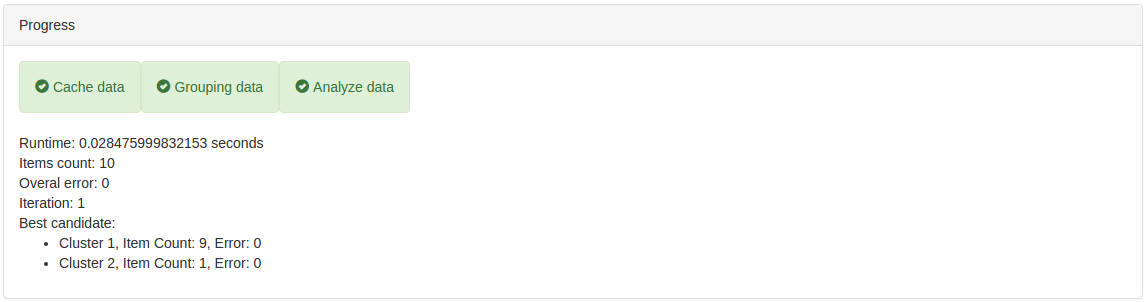
\includegraphics[width=1\textwidth]{images/tc11-kprototype-1}
		\caption{Generelle Informationen}
		\label{fig:testingfazit:testing:testcases:11-2-1}
	\end{subfigure} \\
	\begin{subfigure}[t]{1\textwidth}
		\centering
		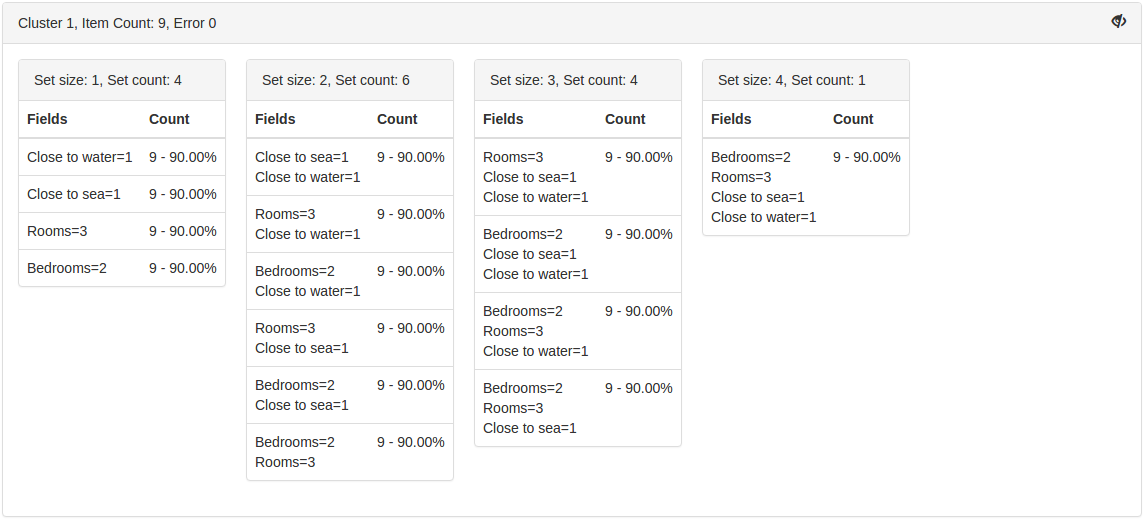
\includegraphics[width=1\textwidth]{images/tc11-kprototype-2}
		\caption{Cluster 1}
		\label{fig:testingfazit:testing:testcases:11-2-2}
	\end{subfigure}
	\begin{subfigure}[t]{1\textwidth}
		\centering
		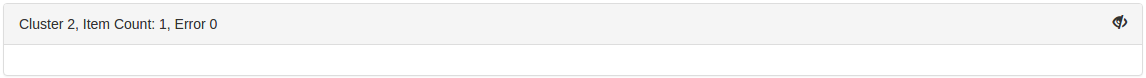
\includegraphics[width=1\textwidth]{images/tc11-kprototype-3}
		\caption{Cluster 2}
		\label{fig:testingfazit:testing:testcases:11-2-3}
	\end{subfigure}
	\caption{TC11-2 - Ausgabe des Programmes - Resultat des k-prototype Algorithmus}
	\label{fig:testingfazit:testing:testcases:11-2}
\end{figure}

\begin{longtable}{ | l | l | l | l |} 	
	\hline 
	\rowcolor{tableheadcolor}
	\multicolumn{4}{|l|}{\bfseries ID: TC12-1 DBSCAN} \\ \hline 
	Datebquelle & \multicolumn{3}{|l|}{\cref{app:testdatenquellen:12}} \\ \hline 
	Dateneinschränkung & \multicolumn{3}{|l|}{Keine} \\ \hline 
	
	\rowcolor{tableheadcolor}
	\multicolumn{4}{|l|}{\bfseries Erwartetes Resultat} \\ \hline 
	Noise Punkte & \multicolumn{3}{|l|}{1} \\ \hline 
	
	% ----------------------------------------------		
	\multicolumn{4}{|l|}{\textbf{Cluster 1}} \\ \cline{2-4} 
	& Grösse & \multicolumn{2}{|l|}{4} \\ \cline{2-4} 
	&& Attributmenge & Anzahl \\ \cline{2-4} 
	
	& 1er-Attributmenge & \tabitem Nahe am Meer & 4 \\ \hline
		
	% ----------------------------------------------		
	\multicolumn{4}{|l|}{\textbf{Cluster 1}} \\ \cline{2-4} 
	& Grösse & \multicolumn{2}{|l|}{5} \\ \cline{2-4} 
	&& Attributmenge & Anzahl \\ \cline{2-4} 
	
	& 1er-Attributmenge & \tabitem Aircondition & 4 \\ \cline{3-4} 
	& & \tabitem Wochenpreis=günstig & 3 \\ \cline{3-4} 
	& & \tabitem Anzahl Zimmer=9 & 3 \\ \cline{3-4} 
	& & \tabitem Anzahl Schlafzimmer=8 & 3 \\ \cline{2-4} 
	
	& 2er-Attributmenge & \tabitem Anzahl Zimmer=9 & 3 \\
	& & \tabitem Wochenpreis=günstig & \\ \hline
		
		
	\rowcolor{tableheadcolor}
	\multicolumn{4}{|l|}{\bfseries Tatsächliches Resultat} \\ \hline 
		
	% ----------------------------------------------		
	\multicolumn{4}{|l|}{\textbf{Cluster 1}} \\ \cline{2-4} 
	& Grösse & \multicolumn{2}{|l|}{4} \\ \cline{2-4} 
	&& Attributmenge & Anzahl \\ \cline{2-4} 
	
	& 1er-Attributmenge & \tabitem Nahe am Meer & 4 \\ \hline
		
	% ----------------------------------------------		
	\multicolumn{4}{|l|}{\textbf{Cluster 1}} \\ \cline{2-4} 
	& Grösse & \multicolumn{2}{|l|}{5} \\ \cline{2-4} 
	&& Attributmenge & Anzahl \\ \cline{2-4} 
	
	& 1er-Attributmenge & \tabitem Aircondition & 4 \\ \cline{3-4} 
	& & \tabitem Wochenpreis=günstig & 3 \\ \cline{3-4} 
	& & \tabitem Anzahl Zimmer=9 & 3 \\ \cline{3-4} 
	& & \tabitem Anzahl Schlafzimmer=8 & 3 \\ \cline{2-4} 
	
	& 2er-Attributmenge & \tabitem Anzahl Zimmer=9 & 3 \\
	& & \tabitem Wochenpreis=günstig & \\ \hline
		
	\rowcolor{tableheadcolor}
	\multicolumn{4}{|l|}{\bfseries Testergebnis} \\ \hline 
	\multicolumn{4}{|l|}{\cellcolor{green!25}} \\ \hline 

	\caption{TC12-1 Auswertung vom DBSCAN Algorithmus}
	\centering
	\label{fig:testingfazit:testing:testcases:12:1}
\end{longtable}
\begin{figure}[H]
	\begin{subfigure}[t]{1\textwidth}
		\centering
		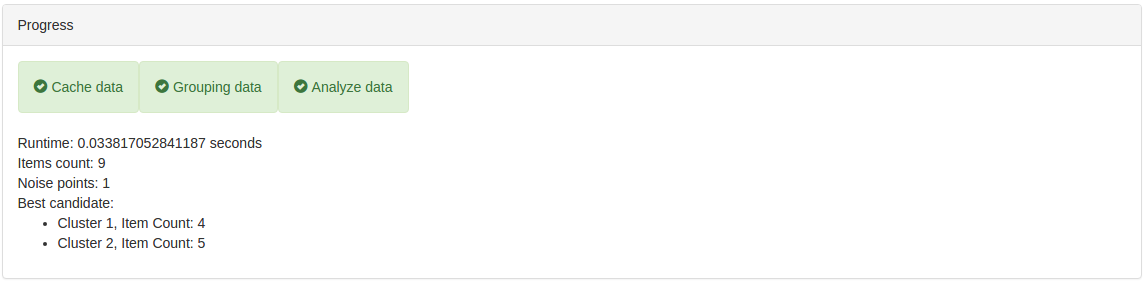
\includegraphics[width=1\textwidth]{images/tc12-dbscan-1}
		\caption{Generelle Informationen}
		\label{fig:testingfazit:testing:testcases:12-1-1}
	\end{subfigure} \\
	\begin{subfigure}[t]{1\textwidth}
		\centering
		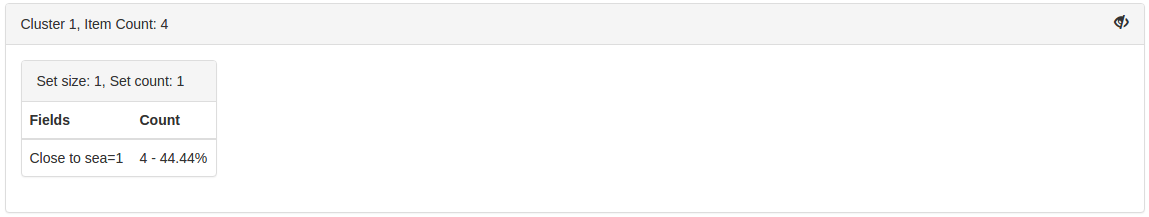
\includegraphics[width=1\textwidth]{images/tc12-dbscan-2}
		\caption{Cluster 1}
		\label{fig:testingfazit:testing:testcases:12-1-2}
	\end{subfigure}\\
	\begin{subfigure}[t]{1\textwidth}
		\centering
		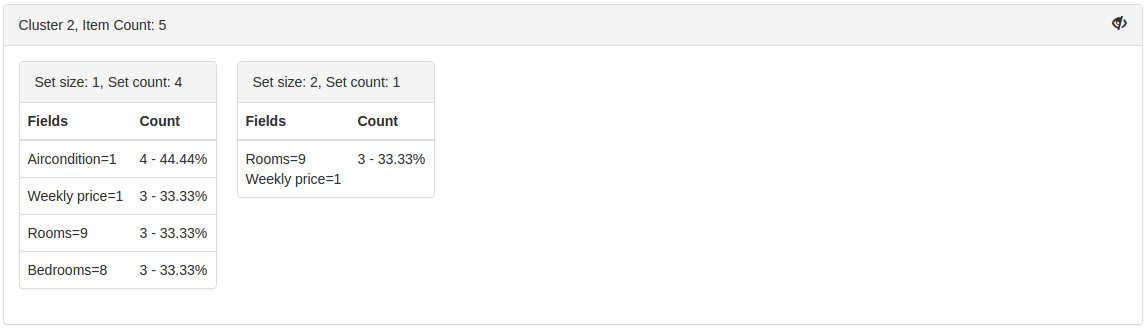
\includegraphics[width=1\textwidth]{images/tc12-dbscan-3}
		\caption{Cluster 2}
		\label{fig:testingfazit:testing:testcases:12-1-3}
	\end{subfigure}
	\caption{TC12 - Ausgabe des Programmes - Resultat des DBSCAN Algorithmus}
	\label{fig:testingfazit:testing:testcases:12-1}
\end{figure}

\begin{longtable}{ | l | l | l | l |} 	
	\hline 
	\rowcolor{tableheadcolor}
	\multicolumn{4}{|l|}{\bfseries ID: TC12-2 k-prototype} \\ \hline 
	Datebquelle & \multicolumn{3}{|l|}{\cref{app:testdatenquellen:12}} \\ \hline 
	Dateneinschränkung & \multicolumn{3}{|l|}{Keine} \\ \hline 
	
	\rowcolor{tableheadcolor}
	\multicolumn{4}{|l|}{\bfseries Erwartetes Resultat} \\ \hline 
		
	% ----------------------------------------------		
	\multicolumn{4}{|l|}{\textbf{Cluster 1}} \\ \cline{2-4}
	& Fehler & \multicolumn{2}{|l|}{6.086575} \\ \cline{2-4}  
	& Grösse & \multicolumn{2}{|l|}{5} \\ \cline{2-4} 
	&& Attributmenge & Anzahl \\ \cline{2-4} 
	
	& 1er-Attributmenge & \tabitem Nahe am Meer & 4 \\ \cline{2-4}
	& & \tabitem Nahe am ÖV (öffentlicher Verkehr) & 3 \\ \hline
		
	% ----------------------------------------------		
	\multicolumn{4}{|l|}{\textbf{Cluster 1}} \\ \cline{2-4} 
	& Fehler & \multicolumn{2}{|l|}{3.090957} \\ \cline{2-4} 
	& Grösse & \multicolumn{2}{|l|}{5} \\ \cline{2-4} 
	&& Attributmenge & Anzahl \\ \cline{2-4} 
	
	& 1er-Attributmenge & \tabitem Aircondition & 4 \\ \cline{3-4} 
	& & \tabitem Wochenpreis=günstig & 3 \\ \cline{3-4} 
	& & \tabitem Anzahl Zimmer=9 & 3 \\ \cline{3-4} 
	& & \tabitem Anzahl Schlafzimmer=8 & 3 \\ \cline{2-4} 
	
	& 2er-Attributmenge & \tabitem Anzahl Zimmer=9 & 3 \\
	& & \tabitem Wochenpreis=günstig & \\ \hline
		
		
	\rowcolor{tableheadcolor}
	\multicolumn{4}{|l|}{\bfseries Tatsächliches Resultat} \\ \hline 
			
	% ----------------------------------------------		
	\multicolumn{4}{|l|}{\textbf{Cluster 1}} \\ \cline{2-4}
	& Fehler & \multicolumn{2}{|l|}{6.086575} \\ \cline{2-4}  
	& Grösse & \multicolumn{2}{|l|}{5} \\ \cline{2-4} 
	&& Attributmenge & Anzahl \\ \cline{2-4} 
	
	& 1er-Attributmenge & \tabitem Nahe am Meer & 4 \\ \cline{2-4}
	& & \tabitem Nahe am ÖV (öffentlicher Verkehr) & 3 \\ \hline
		
	% ----------------------------------------------		
	\multicolumn{4}{|l|}{\textbf{Cluster 1}} \\ \cline{2-4} 
	& Fehler & \multicolumn{2}{|l|}{3.090957} \\ \cline{2-4} 
	& Grösse & \multicolumn{2}{|l|}{5} \\ \cline{2-4} 
	&& Attributmenge & Anzahl \\ \cline{2-4} 
	
	& 1er-Attributmenge & \tabitem Aircondition & 4 \\ \cline{3-4} 
	& & \tabitem Wochenpreis=günstig & 3 \\ \cline{3-4} 
	& & \tabitem Anzahl Zimmer=9 & 3 \\ \cline{3-4} 
	& & \tabitem Anzahl Schlafzimmer=8 & 3 \\ \cline{2-4} 
	
	& 2er-Attributmenge & \tabitem Anzahl Zimmer=9 & 3 \\
	& & \tabitem Wochenpreis=günstig & \\ \hline
		
	\rowcolor{tableheadcolor}
	\multicolumn{4}{|l|}{\bfseries Testergebnis} \\ \hline 
	\multicolumn{4}{|l|}{\cellcolor{green!25}} \\ \hline 
		
	\caption{TC12-2 Auswertung vom k-prototype Algorithmus}
	\centering
	\label{fig:testingfazit:testing:testcases:12:2}
\end{longtable}
\begin{figure}[H]
	\begin{subfigure}[t]{1\textwidth}
		\centering
		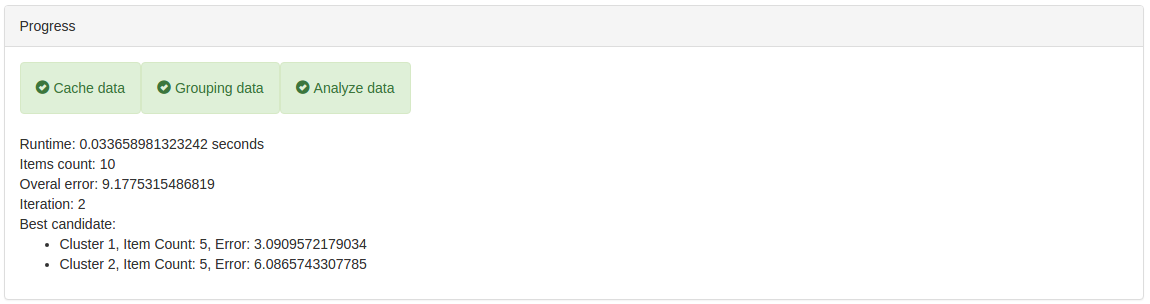
\includegraphics[width=1\textwidth]{images/tc12-kprototype-1}
		\caption{Generelle Informationen}
		\label{fig:testingfazit:testing:testcases:12-2-1}
	\end{subfigure} \\
	\begin{subfigure}[t]{1\textwidth}
		\centering
		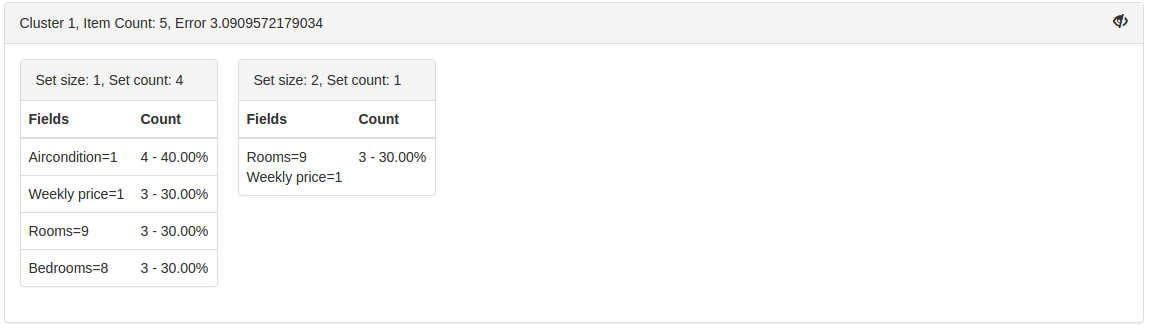
\includegraphics[width=1\textwidth]{images/tc12-kprototype-2}
		\caption{Cluster 1}
		\label{fig:testingfazit:testing:testcases:12-2-2}
	\end{subfigure}
	\begin{subfigure}[t]{1\textwidth}
		\centering
		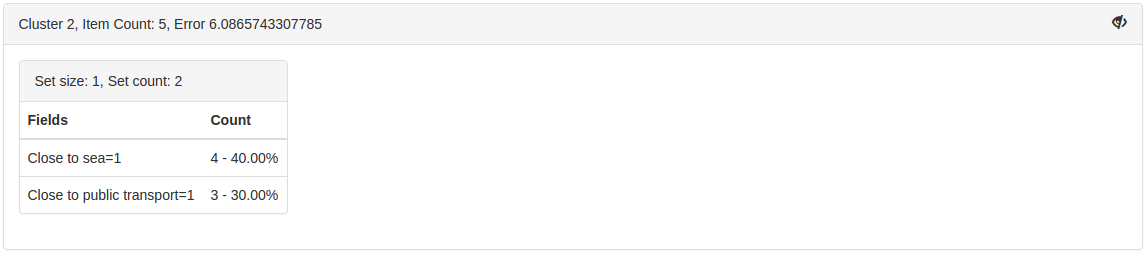
\includegraphics[width=1\textwidth]{images/tc12-kprototype-3}
		\caption{Cluster 2}
		\label{fig:testingfazit:testing:testcases:12-2-3}
	\end{subfigure}
	\caption{TC12-2 - Ausgabe des Programmes - Resultat des k-prototype Algorithmus}
	\label{fig:testingfazit:testing:testcases:12-2}
\end{figure}

\subsection{Hypothesen}
\label{sec:testingfazit:testing:hypothesen}
Im \cref{sec:einleitung:ziel:hypothesen} \nameref{sec:einleitung:ziel:hypothesen} sind Hypothesen aufgestellt worden welche auf ihre Richtigkeit geprüft wurden. Nachfolgend wird das Resultat vorgestellt.

%"`"'
\paragraph{Hypothese 1: "`Die meisten Kunden von Interhome kommen aus der Schweiz oder Frankreich"'} Durch eine Einschränkung der analysierten Attribute des Apriori Algorithmus auf das Herkunftsland des Kunden wurde diese Hypothese bestätigt. 20.94\% aller Buchungen wurden von Schweizer getätigt und 18.58\% von Franzosen. Das Resultat der Apriori Analyse wird in \cref{fig:testingfazit:testing:hypothesen:hypothese1} gezeigt. Die erste Spalte stellt das Attribut dar. "`Object Country"' ist das Land wo das Objekt steht, "`=switzerland"' sagt es liegt in der Schweiz. In der zweiten Spalte wird die Anzahl der Buchungen gezeigt, welche zum Beispiel das Attribut "`Object Country=switzerland"' besitzen, sowie eine Prozentzahl. Diese gibt an wie viele Buchungen dieses Attribut besitzen verglichen mit allen analysierten Instanzen.

\begin{figure}[H]
	\RawFloats
	\centering
	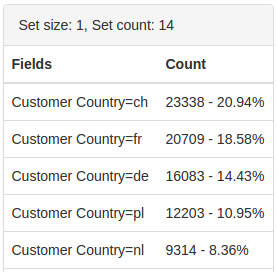
\includegraphics[width=0.5\textwidth]{images/hypothese1}
	\caption{Kunden von Interhome gruppiert nach Land}
	\label{fig:testingfazit:testing:hypothesen:hypothese1}
\end{figure}

\paragraph{Hypothese 2: "`Die meisten Buchungen werden für die Schweiz und für Frankreich getätigt"'} Das Resultat des Apriori Algorithmus wurde für die Auswertung dieser Hypothese eingeschränkt, so dass nur der Standort des Objektes analysiert wird. Als Filter wurde gesetzt dass die Buchung aus der Schweiz stammen muss. Dadurch konnte die Hypothese bestätigt werden. 19.92\% aller Buchungen wurde für Objekte in der Schweiz getätigt, und 13.97\% für deren aus Frankreich.

\begin{figure}[H]
	\RawFloats
	\centering
	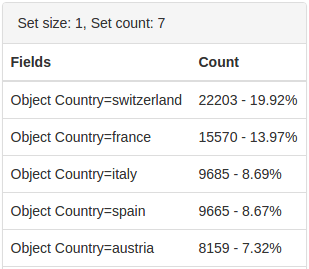
\includegraphics[width=0.5\textwidth]{images/hypothese2}
	\caption{Buchungen von Interhome gruppiert nach Land}
	\label{fig:testingfazit:testing:hypothesen:hypothese2}
\end{figure}

\paragraph{Hypothese 3: "`Schweizer Kunden buchen meistens Objekte in der Schweiz."'} Eingeschränkt wurden die Attribute hier auf den Standort des Objektes. Zusätzlich wurde ein Filter gesetzt auf die Herkunft des Kunden. Als Resultat gab das Programm aus, dass 49.24\% aller Schweizer ein Objekt in der Schweiz buchen. Abgeschlagen auf dem zweiten Platz rangiert Frankreich mit 7.34\% und danach Italien mit 6.99\%. Die Hypothese ist somit bestätigt.

\begin{figure}[H]
	\RawFloats
	\centering
	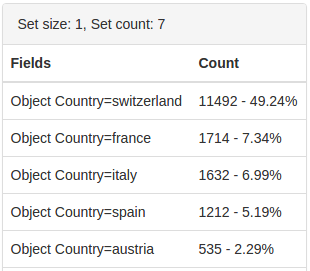
\includegraphics[width=0.5\textwidth]{images/hypothese3-1}
	\caption{Buchungen von Interhome welche von Schweizer getätigt wurden, gruppiert nach Land}
	\label{fig:testingfazit:testing:hypothesen:hypothese3:1}
\end{figure}

Es ist generell gültig, dass Kunden meistens ein Ferienhaus im eigenen Land buchen. Jedoch ist es nirgends so extrem wie in der Schweiz. Franzosen buchen mit 32.20\% am meisten Objekte in Frankreich und mit 16.50\% in Spanien. Italiener buchen zu 18.01\% Objekte in Italien und 17.11\% in Spanien.

\begin{figure}[H]
	\begin{subfigure}[t]{0.4\textwidth}
		\centering
		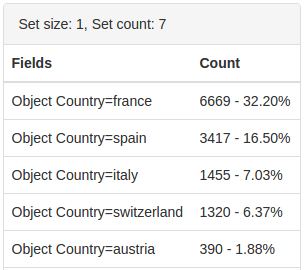
\includegraphics[width=1\textwidth]{images/hypothese3-2}
		\caption{Franzosen}
		\label{fig:testingfazit:testing:hypothesen:hypothese3:2:1}
	\end{subfigure} 
	\begin{subfigure}[t]{0.4\textwidth}
		\centering
		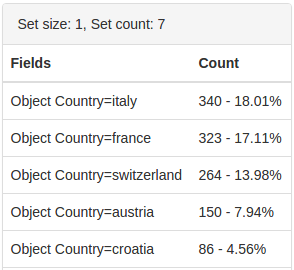
\includegraphics[width=1\textwidth]{images/hypothese3-3}
		\caption{Italiener}
		\label{fig:testingfazit:testing:hypothesen:hypothese3:2:2}
	\end{subfigure}
	\caption{Buchungen von Interhome welche von anderen Nationen getätigt wurden.}
	\label{fig:testingfazit:testing:hypothesen:hypothese3:2}
\end{figure}

\paragraph{Hypothese 4: "`Bei Destinationen mit Meer Anschluss werden öfters Objekte mit mehreren Reisenden gebucht"'} Um diese Hypothese zu überprüfen werden verschiedene Destinationen miteinander verglichen. Benötigt werden Orte am Meer und solche im Landes inneren. Es werden deshalb zuerst Destinationen ermittelt und danach die Durchschnitte der Anzahl \gls{pax} verglichen. Sind durchschnittlich mehr Buchungen mit 2 Reisenden und weniger mit höheren \gls{pax}-Anzahlen vorhanden ist die Hypothese bestätigt.

Es wurden die fünf meist gebuchten Regionen ausfindig gemacht, welche nahe am Strand sind. Dies konnte mit dem Proof of Concept gemacht werden. Dazu wurde die Ortschaft von allen Buchungen analysiert, bei denen das Objekt nahe am Strand liegt. Das Resultat dieser Analyse ist in \cref{sec:testingfazit:testing:hypothesen:1} abgebildet. Die \% Spalte zeigt wie häufig die Ortschaft in der Datenmenge vorhanden ist.

\begin{table}[H] 
	\caption{Häufigkeit der Ortschaften von Buchungen nahe Strand}
	\centering
	\label{sec:testingfazit:testing:hypothesen:1}
	\begin{tabular}{ | l | l | } 
		\hline 
		\rowcolor{tableheadcolor}
		\bfseries Ortschaft & \bfseries \% \\ \hline 
		Spanien - Dénia & 1.84\% \\ \hline 
		Frankreich - Cap d'Agde & 1.58\% \\ \hline 
		Spanien - Llançà & 1.35\% \\ \hline 
		Kroatien - Zadar & 1.14\% \\ \hline 
		Frankreich - Cannes & 1.05\% \\ \hline 
	\end{tabular}
\end{table}

Anschliessend wurde für diese Ortschaften die Häufigkeiten der Anzahl von Passagieren ermittelt. Also wie viele Buchungen wurden mit 2 \gls{pax} getätigt, wie viele mit 3 \gls{pax}, wie viele mit 4 \gls{pax}, etc. Das Resultat wird in \cref{sec:testingfazit:testing:hypothesen:2} gezeigt. Die Kolonne "`\#-PAX"' stellt die Anzahl der Reisenden dar. Die Kolonne "`\%"' die Häufigkeit, wie oft die \gls{pax} Anzahl vorhanden ist in allen Buchungen, bei welchen das Objekt nahe am Meer liegt.

%Man sieht dass am häufigsten 2 oder 4 Reisende vorhanden sind. Zwei \gls{pax} sind sicher keine Familie. Steigt die 
%
%
%hinterlegt und vier Passagiere \colorbox{green!25}{grün}. Erwartet wird dass grüne Felder eine möglichst hohe Zahl haben, und rote eine niedrigere. 3 Reisende werden nicht verwendet da dies genau so gut Familien wie Reisegruppen sein können, und für Buchungen mit 5 bis 6 \gls{pax} sind zu wenige Instanzen vorhanden. Die Werten von 2 und 4 Reisenden werden nachher mit denen von Buchungen verglichen, welche nicht am Strand liegen. Sind die grünen Felder generell höher bei Buchungen am Strand, so gilt die Hypothese als möglich. Um sie endgültig zu bestätigen müssten mehr Informationen gesammelt werden als in dieser Arbeit vorhanden sind. Die Hypothese besagt, dass Familien mit Kindern öfters ans Meer reisen. 4 \gls{pax} jedoch müssen nicht zwingend Familien sein. Die These kann demnach widerlegt werden, denn 2 Reisende sind definitiv keine Familie mit Kindern, jedoch ist eine definitive Bestätigung nicht möglich. 

\begin{table}[H] 
	\caption{Häufigkeit der Anzahl Reisenden pro Buchung für Ortschaften am Meer}
	\centering
	\label{sec:testingfazit:testing:hypothesen:2}
	\begin{tabular}{ | l | l | l | } 
		\hline 
		\rowcolor{tableheadcolor}
		\bfseries Ortschaft & \bfseries \#-PAX & \bfseries \% \\ \hline 
		Spanien - Dénia & 4 & 37.32\% \\ \cline{2-3} 
		 & 2 & 26.17\% \\ \cline{2-3}
		 & 3 & 18.42\% \\ \cline{2-3} 
		 & 5 & 7.43\% \\ \cline{2-3}
		 & 6 & 5.98\% \\ \hline 
		Frankreich - Cap d'Agde & 2 & 32.00\% \\ \cline{2-3} 
		 & 4 & 27.11\% \\ \cline{2-3}
		 & 3 & 21.78\% \\ \cline{2-3} 
		 & 5 & 8.89\% \\ \cline{2-3}
		 & 6 & 6.22\% \\ \hline 
		Spanien - Llançà & 4 & 32.24\% \\ \cline{2-3}
		& 2 & 27.32\% \\ \cline{2-3} 
		& 3 & 16.12\% \\ \cline{2-3}
		& 5 & 8.2\% \\ \cline{2-3}
		& 6 & 5.19\% \\ \hline 
		Kroatien - Zadar & 4 & 31.25\% \\ \cline{2-3}
		& 2 & 18.42\% \\ \cline{2-3} 
		& 5 & 15.79\% \\ \cline{2-3}
		& 3 & 14.80\% \\ \cline{2-3}
		& 6 & 8.22\% \\ \hline 
		Frankreich - Cannes & 2 & 46.72\% \\ \cline{2-3} 
		& 4 & 21.52\% \\ \cline{2-3}
		& 3 & 17.06\% \\ \cline{2-3} 
		& 5 & 3.15\% \\ \cline{2-3}
		& 6 & 1.84\% \\ \hline 
	\end{tabular}
\end{table}

Als Vertreter der Destinationen ohne Meeresanschluss wurden Paris, Wien, Dittishausen, Krakau und Prag gewählt. Sie wurden ausgesucht weil sie sind im Landes inneren sind und viele Buchungen besitzen. 
\begin{table}[H] 
	\caption{Häufigkeit der Anzahl Reisenden pro Buchung für Ortschaften welche nicht am Meer liegen}
	\centering
	\label{sec:testingfazit:testing:hypothesen:3}
	\begin{tabular}{ | l | l | l | } 
		\hline 
		\rowcolor{tableheadcolor}
		\bfseries Ortschaft & \bfseries \#-PAX & \bfseries \% \\ \hline 
		Frankreich - Paris & 2 & 45.83\% \\ \cline{2-3} 
		 & 4 & 26.21\% \\ \cline{2-3}
		 & 3 & 14.76\% \\ \cline{2-3} 
		 & 5 & 5.44\% \\ \cline{2-3}
		 & 6 & 2.33\% \\ \hline 
		Österreich - Wien & 2 & 36.07\% \\ \cline{2-3} 
		 & 4 & 29.18\% \\ \cline{2-3}
		 & 3 & 19.10\% \\ \cline{2-3} 
		 & 5 & 10.08\% \\ \cline{2-3}
		 & 6 & 2.65\% \\ \hline 
		Deutschland - Dittishausen & 2 & 37.38\% \\ \cline{2-3}
		& 4 & 25.54\% \\ \cline{2-3} 
		& 3 & 19.08\% \\ \cline{2-3}
		& 5 & 7.38\% \\ \cline{2-3}
		& 6 & 4.31\% \\ \hline 
		Polen - Krakau & 4 & 38.46\% \\ \cline{2-3}
		& 2 & 17.31\% \\ \cline{2-3} 
		& 6 & 15.38\% \\ \cline{2-3}
		& 5 & 15.38\% \\ \cline{2-3}
		& 3 & 9.62\% \\ \hline 
		Tschechien - Prag & 4 & 45.26\% \\ \cline{2-3} 
		& 3 & 20.44\% \\ \cline{2-3}
		& 2 & 16.06\% \\ \cline{2-3} 
		& 5 & 9.49\% \\ \cline{2-3}
		& 6 & 8.03\% \\ \hline 
	\end{tabular}
\end{table}

Die \cref{sec:testingfazit:testing:hypothesen:3:2} zeigt die Durchschnitte der Anzahl der Reisenden auf.
\begin{table}[H] 
	\caption{Durchschnittliche Häufigkeit der verschiedenen }
	\centering
	\label{sec:testingfazit:testing:hypothesen:3:2}
	\begin{tabular}{ | c | c | c | } 
		\hline 
		\rowcolor{tableheadcolor}
		\bfseries \#-PAX & \bfseries Meer & \bfseries Landesinnere \\ \hline 		
		2 & 30.13\% & 30.53\% \\ \hline
		3 & 17.64\% & 16.60\% \\ \hline
		4 & 29.89\% & 32.94\% \\ \hline
		5 & 8.69\% & 9.55\% \\ \hline
		6 & 5.48\% & 6.54\% \\ \hline
	\end{tabular}
\end{table}

Die Werte für zwei \gls{pax} ist mit 30.13\% gegenüber 30.53\% annähernd stabil. Dreis Reisende gehen eher ans Meer (17.64\% gegenüber 16.50\%). Bei vier, fünf und sechs Passagieren ist der Wert höher in Destinationen im Landesinneren als am Meer. Am spannendsten sind vier \gls{pax}, da es mit rund 30\% die häufigste Reisengruppengrösse darstellt. Da dieser Wert jedoch im Landesinneren 3\% Punkte höher ist, gilt die Hypothese als widerlegt.

In diesem Bereich würde es sich jedoch anbieten, die Nachforschungen noch etwas zu verstärken. Die Beschreibung der Hypothese besagt, dass Familien eher ans Meer gehen. Grössere Reisegruppen müssen aber nicht zwingend eine Familie sein. Man könnte zum Beispiel Analysieren, ob Gruppen mit zwei Erwachsenen und 1 bis mehrere Kindern sich anders verhalten als Gruppen von nur Erwachsenen Personen.

\paragraph{Hypothese 5: "`Schweizer Buchungen in Skiregionen haben mehrheitlich (80\%) die Eigenschaft dass sie nahe am Skilift oder am öffentlichem Verkehr liegen"'} Zuerst werden die 5 grössten Skiregionen ermittelt. Dazu wird der Proof of Concept verwendet. Es werden Schweizer Ortschaften gesucht und die Häufigkeit der Region gezählt mittels dem Apriori Algorithmus. Anschliessen die fünf Top-Ortschaften aus dem Resultat ausgesucht welche ein Skigebiet besitzen. Das Resultat der Apriori Analyse ist in \cref{sec:testingfazit:testing:hypothesen:4} aufgeführt. \colorbox{green!25}{Grün} hinterlegt sind diejenigen Regionen, welche ein Skigebiet besitzen und deshalb weiterverwendet werden. Anschliessend wird für jede Region mittels Apriori Analyse ermittelt, wie viele Objekte entweder nahe am Skigebiet oder nahe am Öffentlichen verkehr liegen. 

\begin{table}[H] 
	\caption{Häufigkeit der Ortschaften von Buchungen nahe Strand}
	\centering
	\label{sec:testingfazit:testing:hypothesen:4}
	\begin{tabular}{ | l | l | } 
		\hline 
		\rowcolor{tableheadcolor}
		\bfseries Ortschaft & \bfseries \% \\ \hline 
		\cellcolor{green!25}Wallis - Nendaz & \cellcolor{green!25}13.10\% \\ \hline 
		\cellcolor{green!25}Wallis - Zermatt & \cellcolor{green!25}6.90\% \\ \hline 
		\cellcolor{green!25}Wallis - Crans-Montana & \cellcolor{green!25}6.66\% \\ \hline 
		\cellcolor{green!25}Bern - Grindelwald & \cellcolor{green!25}6.49\% \\ \hline 
		Tessin - Ascona & 5.47\% \\ \hline 
		Wallis - Ovronnaz & 4.31\% \\ \hline 
		\cellcolor{green!25}Waadt - Villars-sur-Ollon & \cellcolor{green!25}4.29\% \\ \hline
	\end{tabular}
\end{table}

\begin{figure}[H]
	\begin{subfigure}[t]{0.8\textwidth}
		\centering
		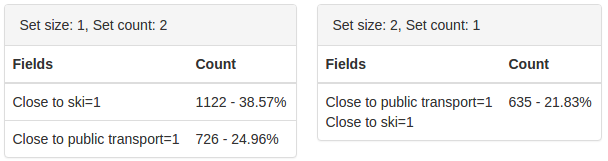
\includegraphics[width=1\textwidth]{images/hypothese5-nendaz}
		\caption{Nendaz}
		\label{sec:testingfazit:testing:hypothesen:5:1}
	\end{subfigure}  \\
	\begin{subfigure}[t]{0.8\textwidth}
		\centering
		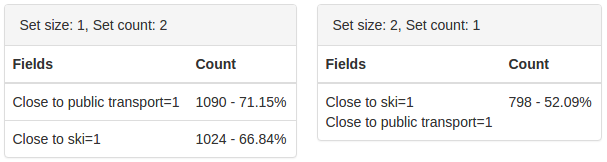
\includegraphics[width=1\textwidth]{images/hypothese5-zermatt}
		\caption{Zermatt}
		\label{sec:testingfazit:testing:hypothesen:5:2}
	\end{subfigure} \\
	\begin{subfigure}[t]{0.8\textwidth}
		\centering
		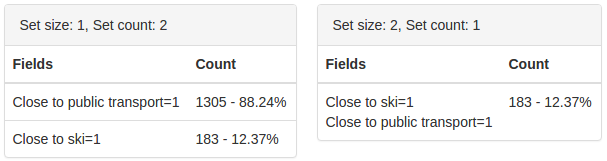
\includegraphics[width=1\textwidth]{images/hypothese5-crans-montana}
		\caption{Crans-Montana}
		\label{sec:testingfazit:testing:hypothesen:5:3}
	\end{subfigure} \\
	\begin{subfigure}[t]{0.8\textwidth}
		\centering
		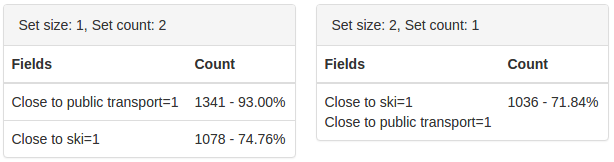
\includegraphics[width=1\textwidth]{images/hypothese5-grindelwald}
		\caption{Grindelwald}
		\label{sec:testingfazit:testing:hypothesen:5:4}
	\end{subfigure} \\
	\begin{subfigure}[t]{0.8\textwidth}
		\centering
		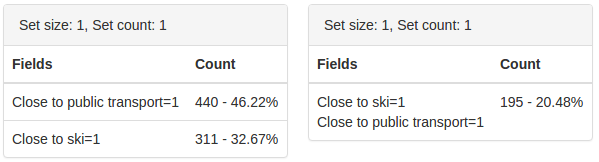
\includegraphics[width=1\textwidth]{images/hypothese5-villars}
		\caption{Villars-sur-Ollon}
		\label{sec:testingfazit:testing:hypothesen:5:5}
	\end{subfigure}
	\caption{Analyse der Skiregionen auf Distanz zum Skilift und zum öffentlichen Verkehr mit dem Apriori Algorithmus}
	\label{sec:testingfazit:testing:hypothesen:5}
\end{figure}

Bei Crans-Montana mit 88.24\% und Grindelwald 93.00\% der Buchungen in der nähe des öffentlichen Verkehrs (ÖV) ist die Hypothese erfüllt. 

In Zermatt sind 71.15\% nahe ÖV, 66.84\% nahe dem Skilift und 52.09\% in der nähe von beiden. Wenn man $66.84 - 52.09$ rechnet erhält an 14.75\%. Dies sind die Buchungen die nur in der nähe von einem Skigebiet liegen, jedoch nicht in der nähe der ÖV. Zählt man diese 14.75\% zu den 71.15\%, so erhält 85.9\% und damit alle Objekte die nahe Skilift und/oder nahe ÖV liegen. Somit ist die Hypothese auch für Zermatt erfüllt.

In Villars-sur-Ollon sind 58.41\% ($32.67-20.48+46.22$)  und in Nendaz 41.7\% ($24.96-21.83+38.57$) in der Nähe vom Skilift und/oder ÖV und die Hypothese damit nicht erfüllt.

Abschliessend kann die Hypothese widerlegt werden. Sie ist sicherlich richtig für einige Skigebiete, jedoch nicht für alle.

\paragraph{Hypothese 6: "`Zu kalten Jahreszeiten wird von Schweizern mehr Regionen am Meer gebucht als im Sommer."'} Analysiert wird diese Hypothese mit dem Apriori Algorithmus. Filtriert wird nach Buchungen aus der Schweiz. Als Resultate werden die Region und Ortschaft der Buchungen verwendet. Das Resultat dieser Anylse ist in \cref{fig:testingfazit:testing:hypothesen:6} aufgeführt. Die Kolonne "`\#-Buchungen"' listet die Anzahl der Instanzen auf, welche im gegebenen Monat gebucht wurden.

\begin{table}[H] 
	\caption{Häufigkeit der Regionen und Ortschaften gruppiert nach Buchungsmonat}
	\centering
	\label{fig:testingfazit:testing:hypothesen:6}
	\begin{tabular}{ | l | l | l | l | } 
		\hline 
		\rowcolor{tableheadcolor}
		\bfseries Monat(e) & \bfseries \#-Buchungen & \bfseries Region/Ortschaft & \bfseries \% \\ \hline 
		Januar & 2942 & Region: Cote d'Azur & 2.33\% \\ \cline{3-4} 
		 & & Ort: Leukerbad & 1.95\% \\ \cline{3-4}
		 & & Region: Costa Blanca & 1.92\% \\ \cline{3-4}
		 & & Region: Toskana & 1.47\% \\ \hline
		 Juli & 1892 & Region: Cote d'Azur & 4.02\% \\ \cline{3-4} 
 		 & & Region: Costa Blanca & 2.06\% \\ \cline{3-4}
 		 & & Ort: Leukerbad & 1.90\% \\ \cline{3-4}
 		 & & Region: Toskana & 1.74\% \\ \hline
		 Dezember & 1539 & Region: Cote d'Azur & 2.47\% \\ \cline{3-4} 
		 & & Ort: Leukerbad & 1.62\% \\ \cline{3-4}
 		 & & Region: Costa Blanca & 1.43\% \\ \cline{3-4}
 		 & & Region: Toskana & 0.97\% \\ \hline
		 Dez/Jan/Feb & 6718 & Region: Cote d'Azur & 2.75\% \\ \cline{3-4} 
 		 & & Region: Costa Blanca & 2.01\% \\ \cline{3-4}
 		 & & Ort: Leukerbad & 1.73\% \\ \cline{3-4}
 		 & & Region: Toskana & 1.58\% \\ \hline
		 Jul/Aug/Sep & 6090 & Region: Cote d'Azur & 3.22\% \\ \cline{3-4} 
		 & & Ort: Leukerbad & 2.63\% \\ \cline{3-4}
 		 & & Region: Costa Blanca & 2.00\% \\ \cline{3-4}
 		 & & Region: Toskana & 1.95\% \\ \hline		 
	\end{tabular}
\end{table}

Als warme/Sommer wurden Juli, August und September definiert sowie Dezember, Januar und Februar als kalte/Winter Monate. Aufgeführt in der Tabelle oben sind die Regionen Cote d'Azur, Costa Blanca und Toskana. Dabei handelt es sich um die Top-Regionen der Analyse welche bekannt sind für schönes und warmes Wetter. Zusätzlich ist der Ort Leukerbad ersichtlich, welcher bekannt ist für die Therme. Es wird zusätzlich noch analysiert, ob die warmen Bäder der Therma öfters im Winter gebucht werden als im Sommer.

Aus der Auswertung des Proof of Concepts ist ersichtlich, dass im Juli und im Sommer (Juli, August und September) die aufgeführten Regionen und das Leukerbad mehr gebucht wird als im Winter. Das ist das gegenteilige Resultat der Hypothese, womit diese widerlegt ist.

\paragraph{Hypothese 7: "`Anfang des Jahres werden teurere Objekte gebucht als Mitte oder Ende des Jahres"'} Verglichen werden hier die Wochenpreise zusammengefasst nach Monat. Analysiert werden alle Buchungen. Es werden demnach keine Filter angewendet.
\begin{table}[H] 
	\caption{Häufigkeit der Wochenpreisen gruppiert nach Buchungsmonat}
	\centering
	\label{fig:testingfazit:testing:hypothesen:7}
	\begin{tabular}{ | l | l | l | l | } 
		\hline 
		\rowcolor{tableheadcolor}
		\bfseries Monat(e) & \bfseries \#-Buchungen & \bfseries Wochenpreis & \bfseries \% \\ \hline 
		Januar & 14041 & Budget & 33.77\% \\ \cline{3-4} 
		 & & Luxury & 28.01\% \\ \hline
		 Februar & 11328 & Budget & 35.20\% \\ \cline{3-4} 
 		 & & Luxury & 28.72\% \\ \hline
		 Juni & 8969 & Budget & 31.05\% \\ \cline{3-4} 
 		 & & Luxury & 30.45\% \\ \hline
		 November & 6697 & Budget & 31.58\% \\ \cline{3-4}
 		 & & Luxury & 30.36\% \\ \hline
		 Dezember & 6860 & Budget & 33.69\% \\ \cline{3-4} 
 		 & & Luxury & 28.00\% \\ \hline		 
	\end{tabular}
\end{table}

Die teuren/Luxus Buchungen sind am meisten Vertreten im Juni und November, und nicht am Anfang Jahr wie erwartet. Jedoch ist ersichtlich, dass die Anzahl der Buchungen im Januar deutlich am höchsten ist mit 14'041 und kontinuierlich abnehmen. Es werden demnach nicht teurere Buchungen anfang des Jahres getätigt, sondern mehr. Diese Hypothese muss somit widerlegt werden. Die gewonnen Erkenntnisse sind dennoch spannend. 

\section{Fazit}
Die Anforderung dieser Arbeit war es, Buchungen von Interhome nach Häufigkeit der Attribute zu analysieren und damit Muster aufzuzeigen. Um dieses Ziel zu erreichen wurden Hypothesen aufgestellt und Algorithmen des Data Mining gesucht, welche die Fragestellungen beantworten können. Es wurde entschieden, den Apriori Algorithmus einzusetzen, da er genau für solche Problemstellungen ausgelegt ist. Zusätzlich wurden noch die zwei Clustering Algorithmen k-prototype und DBSCAN gewählt, in der Hoffnung dass sie die Resultate der Analyse mittels Apriori verbessern. 

Die Auswertung der Hypothesen (siehe \cref{sec:testingfazit:testing:hypothesen} \nameref{sec:testingfazit:testing:hypothesen}) hat gezeigt, dass sich die Auswahl des Apriori Algorithmus bewährt hat. Einzig bei Hypothese 4 gab es Probleme bei der Auswertung wegen des Begriffes "`Familie"'. Die Datenbasis kennt nur \gls{pax} und der Algorithmus weiss nicht, ob es sich um eine Reisegruppe oder eine Familie handelt. Durch eine Analyse welche zwischen Erwachsenen und Kinder unterscheiden würde könnten die Resultate noch verfeinert werden. Da kann noch mehr Nachgeforscht werden. Verhalten sich Reisende mit Kindern anders als Gruppen von nur Erwachsenen?

Die funktionalen Anforderungen aus \cref{sec:anforderungsanalyse:funktionaleanforderung} \nameref{sec:anforderungsanalyse:funktionaleanforderung} wurden alle umgesetzt. Eine Häufigkeitsanalyse kann gemäss FA1 auf allen Instanzen durchgeführt werden und laut FA3 auch auf einer Untermenge. Die vorgegebene Nachvollziehbarkeit von FA2 ist auch gegeben. Es wird für jede Apriori Analyse die Anzahl der Buchungen sowie die Prozentanzahl an der analysierten Menge angegeben. Um FA4 und FA5 zu erfüllen wurde die "`Explore"' Ansicht erstellt welche alle Stammdaten oder eine Untermenge davon anzeigt. FA6 wird vom Apriori Algorithmus unterstützt. Er zählt die vorkommen von numerischen und kategorischen Attributen. Damit die Clustering Algorithmen mit mixed data types umgehen können wurde eine Distanzmessung definiert welche dies beherrscht (siehe \cref{sec:konzept:anwendungderalgorithmen:distanzmessung} \nameref{sec:konzept:anwendungderalgorithmen:distanzmessung}). FA7 gibt vor dass der Benutzer die Algorithmen konfigurieren kann (siehe \cref{sec:anforderungsanalyse:funktionaleanforderung} \nameref{sec:anforderungsanalyse:funktionaleanforderung}). Dazu wurde die Ansicht "`Settings"' erstellt.  

Für die Messung der Komplexität der nicht funktionalen Anforderung NFA1 (siehe \cref{sec:anforderungsanalyse:nichtfunktionaleanforderung} \nameref{sec:anforderungsanalyse:nichtfunktionaleanforderung}) wurde das Programm zwei Mitarbeitern der Interhome vorgestellt, welche rasch eigene Analysen starten konnten. Sie benutzten verschiedene Filter und machten Anpassungen an den Einstellungen. Die einzelnen Parameter musste Ihnen jedoch erklärt werden da die Erklärung der Einstellungen nicht sprechend genug waren. Obwohl dies ein kleines Detail ist, trägt es trotzdem wesentlich zur Akzeptanz des Programmes bei. Da ist sicher noch Verbesserdungsbedarf. Um die Modularität der Umsetzung gemäss NFA2 zu gewährleisten wurde bei der Entwicklung versucht das \gls{srp} einzuhalten. Durch den Einsatz von UnitTests wurde ebenfalls eine möglichst starke Kohäsion und eine lose Kopplung angestrebt. Weitere Attribute in der Datenbasis können durch reine Konfigurationsänderungen hinzugefügt werden. Für die Einführung eines neuen Algorithmus muss ein neuer Service erstellt werden, jedoch ist keine Änderung an bestehenden Code nötig. Für die Erweiterbarkeit der Daten gemäss NFA3 müssen neue Daten entsprechend \cref{sec:recherche:datenvorbereitung} \nameref{sec:recherche:datenvorbereitung} vorbereitet werden. Ist eine Lizenz für das RapidMiner Programm vorhanden ist dies durch wenige Klicks erledigt, ansonsten muss eine andere Lösung gefunden werden. Sind die Daten korrekt vorbereitet kann jedoch in der Konfiguration des umgesetzten Programmes die neue Datenbasis eingebunden werden. 

Wie im \cref{sec:proofofconcept:fazit} \nameref{sec:proofofconcept:fazit} erläutert eignet sich der Apriori Algorithmus für die explorative Suche von Mustern. Hauptsache dafür ist dessen Geschwindigkeit und die Einfachheit des Programmes. Die Clustering Algorithmen konnten leider keine hilfreichen Resultate liefern. Wie im \cref{sec:proofofconcept:fazit} \nameref{sec:proofofconcept:fazit} beschrieben ist noch unklar, ob es an den falschen Parameter der Algorithmen liegt. Es wurde eine Hypothese aufgestellt welche jedoch das Verhalten der Clusteralgorithmen erklärt. Dieses würde darauf schliessen, dass es keine klaren Gruppen gibt und die beiden Algorithmen demnach nicht geeignet sind um die Buchungen von Interhome zu analysieren.


%\section{Mögliche Erweiterungen/Verbesserungen}
%Diskretiesierungsschritte \cref{sec:recherche:datenvorbereitung} nach Häufigkeitsanalyse.
%Z.b. die Preise plotten -> man sieht ein peek bei CHF1000/Buchung. +/- 1/3 vom Peek sind die normalen Preise. Darunter Budget, darüber Luxury
%
%\gls{optics} einsetzen um $\epsilon$ bei \gls{dbscan} zu eliminieren.
%
%Hierarchical clustering einsetzen. Allerdings weniger performant und deshalb schlecht fürs explorieren geeignet.
%
%Sockets einsetzen um Polling vom Webbrowser zu vermeiden.

\section{Schlusswort}
Die Apriori Analyse hat sich als hilfreiches Werkzeug für die Attributanalyse der Interhome Buchungsdaten herausgestellt, solange die korrekten Anfragen gestellt werden. Die Clustering Algorithmen konnten hingegen keinen Beitrag zum Ziel dieser Arbeit leisten. Trotzdem wurde durch ihren Einsatz wertvolle Einblicke und ein besseres Verständnis der Datenbasis gewonnen werden. Für den produktiven Einsatz sollte jedoch die Beischreibung der möglichen Einstellungen im Programm noch verständlicher erläutert werden. 